%%%%%%%%%%%%%%%%%%%%%%%%%%%%%%%%%%%%%%%%%%%%%%%%%%%%%%%%%%%%%%%%%%%%%%%%%%%%%%%%
% Template for TISMIR Papers
% 2017 version, based on previous ISMIR conference template
%%%%%%%%%%%%%%%%%%%%%%%%%%%%%%%%%%%%%%%%%%%%%%%%%%%%%%%%%%%%%%%%%%%%%%%%%%%%%%%%

\documentclass{article}

%%%%%%%%%%%%%%%%%%%%%%%%%%%%%%%%%%%%%%%%%%%%%%%%%%%%%%%%%%%%%%%%%%%%%%%%%%%%%%%%
% Sample Document LaTeX packages
%%%%%%%%%%%%%%%%%%%%%%%%%%%%%%%%%%%%%%%%%%%%%%%%%%%%%%%%%%%%%%%%%%%%%%%%%%%%%%%%

\usepackage[utf8]{inputenc}
\usepackage{tismir}
\usepackage{amsmath}
\usepackage[]{hyperref}
\usepackage{url}
\usepackage{graphicx}
\usepackage{booktabs}
\usepackage{subfig}
\usepackage{todonotes}
\usepackage{neuralnetwork}
\usepackage{tikz}
\usetikzlibrary{positioning}
\usepackage{multirow}


\tikzset{%
   neuron missing/.style={
    draw=none, 
    scale=1.5,
    text height=0.333cm,
    execute at begin node=\color{black}$\vdots$
  },
}



\newcommand{\secref}[1]{\mbox{Section~\ref{#1}}}
\newcommand{\chapref}[1]{\mbox{Chapter~\ref{#1}}}
\newcommand{\tabref}[1]{\mbox{Table~\ref{#1}}}
\newcommand{\figref}[1]{\mbox{Figure~\ref{#1}}}


%%%%%%%%%%%%%%%%%%%%%%%%%%%%%%%%%%%%%%%%%%%%%%%%%%%%%%%%%%%%%%%%%%%%%%%%%%%%%%%%
% Title and Author information
%%%%%%%%%%%%%%%%%%%%%%%%%%%%%%%%%%%%%%%%%%%%%%%%%%%%%%%%%%%%%%%%%%%%%%%%%%%%%%%%

\title{MIDI2vec: Learning MIDI Embeddings for Reliable Prediction of Symbolic Music Metadata}
%
\author{%
First Author1\thanks{University One, Campus Rd. 3, 12345 Mirland},%
~Second Author2\thanks{Research Institute Two, Campus Rd. 4, 12345 Flatland},%
~and Third Author3\protect\endnotemark[1]}

\date{}


%%%%%%%%%%%%%%%%%%%%%%%%%%%%%%%%%%%%%%%%%%%%%%%%%%%%%%%%%%%%%%%%%%%%%%%%%%%%%%%%
% Additional Paper Information
%%%%%%%%%%%%%%%%%%%%%%%%%%%%%%%%%%%%%%%%%%%%%%%%%%%%%%%%%%%%%%%%%%%%%%%%%%%%%%%%

% Article Type - Uncomment and modify, if necessary.
% Accepted values: research, overview, and dataset
\type{research}

% Citation in First Page
%
% "Mandatory" (if missing will print the complete list of authors,
% including the \thanks symbols)
\authorref{Author1,~F., Author2,~S., and Author3,~T.}
%
% (Optional)
% \journalyear{2017}
% \journalvolume{V}
% \journalissue{N}
% \journalpages{xx--xx}
% \doi{xx.xxxx/xxxx.xx}

% Remaining Pages (Optional)
%
\authorshort{Author1, Author2 and Author3} %or, e.g., \authorshort{Author1 et al}
\titleshort{MIDI2vec: Learning MIDI Embeddings}

%%%%%%%%%%%%%%%%%%%%%%%%%%%%%%%%%%%%%%%%%%%%%%%%%%%%%%%%%%%%%%%%%%%%%%%%%%%%%%%%
% Document Content
%%%%%%%%%%%%%%%%%%%%%%%%%%%%%%%%%%%%%%%%%%%%%%%%%%%%%%%%%%%%%%%%%%%%%%%%%%%%%%%%

\begin{document}

%%%%%%%%%%%%%%%%%%%%%%%%%%%%%%%%%%%%%%%%%%%%%%%%%%%%%%%%%%%%%%%%%%%%%%%%%%%%%%%%
% Abstract
%%%%%%%%%%%%%%%%%%%%%%%%%%%%%%%%%%%%%%%%%%%%%%%%%%%%%%%%%%%%%%%%%%%%%%%%%%%%%%%%

\twocolumn[{%
%
\maketitleblock
%
\begin{abstract}
% max 250 words 
In the literature, studies on symbolic music have focused on the extraction of several musical features such as the pitch range or rhythmic factors. Recently, embedding strategies have been exploited for representing latent factors in graphs of connected nodes. In this work, we propose MIDI2vec, a new approach for representing MIDI files as vectors based on graph embedding techniques. Our strategy consists of representing the MIDI data as a graph, including the information about tempo, time signature, programs and notes. Next, we run and optimise node2vec for generating embeddings using random walks in the graph. We demonstrate that the resulting vectors can successfully be employed for predicting the musical genre and other metadata such as the composer, the instrument or the movement. In particular, we conduct experiments using those vectors as input to a Feed-Forward Neural Network and we report 
% higher 
comparable accuracy scores in the prediction with respect to other approaches relying purely on symbolic music,
% .
% with the advantage of
avoiding feature engineering and producing highly scalable and reusable models with low dimensionality.
Our proposal has real-world applications in automated metadata tagging for symbolic music, for example in digital libraries for musicology, datasets for machine learning, and knowledge graph completion.

\end{abstract}
%
\begin{keywords}
% Up to six keywords (optional).
symbolic music - metadata - genre prediction - embeddings
\end{keywords}
}]
\saythanks{}

%%%%%%%%%%%%%%%%%%%%%%%%%%%%%%%%%%%%%%%%%%%%%%%%%%%%%%%%%%%%%%%%%%%%%%%%%%%%%%%%
% Main Content Start
%%%%%%%%%%%%%%%%%%%%%%%%%%%%%%%%%%%%%%%%%%%%%%%%%%%%%%%%%%%%%%%%%%%%%%%%%%%%%%%%

\section{Introduction}
\label{sec:introduction}
High-quality metadata is a prerequisite in many music information retrieval (MIR) tasks, like accessing symbolic music collections, music recommender systems and discovery \citep{casey2008content}. Historically, the availability of this metadata has depended on manual human annotation labour, which is typically costly. Consequently, several systems have been proposed that automatically analyse (symbolic) music in order to 
% extract
annotate
high-level features, some being abstract enough to be close to traditional metadata \citep{bogdanov2013essentia}. 
Due to the need of high-quality annotated datasets, these systems have many real-world applications. For example, digital libraries for musicology can use them for automatically tagging metadata, lowering manual tagging costs and improving results of music information retrieval systems. In recently proposed music knowledge graphs \cite{merono2017midi}, these systems could be used to complete missing information in the graph. Another application is in machine learning for music, which needs large amounts of music data annotations that could be provided by such systems, for applications such as data programming \cite{ratner2017data} or weak supervision \cite{ratner2017snorkel} or even music recommender systems based on similarity.

In this work, we focus on symbolic music in MIDI format \citep{midispec} due to its high availability on the Web and its popularity in tasks like music generation \citep{roberts2018}.
% and music knowledge graphs \citep{merono2017midi}.
% \todo[inline]{Albert: make argument about possible applications if we had large scale performant reliable metadata classification}
This popularity has also given birth to large MIDI datasets that need, besides high-quality annotations, scalable approaches producing them.
% To address your question of whether metadata classification in MIDI files is needed at all, we have extended our motivation in Section 1 referencing recent works presented in ISMIR and ISWC that express the clear need for automated, reliable and scalable symbolic music metadata classification for various MIR tasks.
Despite their natural fit as a transcription format for music, MIDI files alone have a number of limitations, all concerning the fact that track information (instruments, vocals, metadata) is not standardized and often only implicit \citep{raffel2016}. One way of addressing this is to express MIDI information using RDF and ontologies \citep{merono2017midi}, allowing for the re-use and standardization of missing MIDI metadata at Web scale. The Lakh MIDI dataset \citep{raffel2016} is another important MIR benchmark used in e.g. automatic audio transcription; however, only 31,034 of its 176,581 MIDI files (17.57\%) are aligned with metadata from the Million Song Dataset~\citep{raffel2016thesis}.

%  Lakh dataset: 176,581 midi, of which 31034 are aligned to MSD

Reconstructing this kind of high-level metadata from symbolic musical content, automatically and at scale, is a challenging task due to the existing semantic gap between the desired metadata and low-level music descriptors \citep{celma2008foafing}. One way of addressing this is by analysing the content for predicting higher-level metadata. So far, research has mainly focused on genre \citep{McKay2004,Cataltepe2007}, emotion, and composer \citep{fu2011survey} classification mainly using supervised machine learning techniques. However, traditional machine learning algorithms are limited by the need to perform some feature selection in the so-called feature engineering process \citep{guyon2003introduction}. 

% Feature engineering can be a costly process and can overfit models \citep{guyon2003introduction}. Moreover, some latent or hidden features that lie in the data might be hard, if not impossible, for a human engineer to discover and model 

In order to overcome this, embedding-based methods have been proposed. Embeddings are mappings that transform the symbolic representations of discrete variables (elements which cannot be naturally ordered such as words or songs) into numeric vectors. Each dimension of an embedding vector represents a latent feature which has been automatically learned. Avoiding more expensive representations such as the one-hot encoding, embedding vectors are useful at reducing the dimensionality of the input data of neural networks, a typical choice to address a learning task such as automatic classification. 
Such embedding-based methods have been successfully applied to textual \citep{mikolov2013efficient} and graph data \citep{grover2016node2vec} and notably also on MIDI data for the task of automated music generation through Recurrent Neural Networks (RNN) \citep{huang2016deepmusic,yan2018part} and self-learning techniques such as Variational Autoencoders (VAE) \citep{roberts2018}. Graph embeddings have become a widely used and effective way to represent graph information in a way neural networks can easily process it \citep{ristoski2018rdf2vec}.

Therefore, embedding-based methods seem a good candidate to overcome some of the limitations of feature engineering, which can be a costly process and can overfit models \citep{guyon2003introduction}. Moreover, some latent, hidden features that lie in the data might be hard, if not impossible, for a human engineer to discover and model \citep{wilcke2017knowledge};
some music information tends to be ambiguous and loosely defined (e.g. ``Allegro'', ``Prelude''), and therefore a more fuzzy representation can constitute an advantage;
besides, current feature-engineered methods have pitfalls in scalability with respect to the dataset size and the number of metadata classes to predict \citep{mckay2010datasetslac}. However, feature engineering is still generally faster than learning latent features from data, since it is based on given knowledge; and it is easier to debug because engineered features are human-understandable. Moreover, embeddings can certainly overfit models as well \citep{weng2019overfit}. Therefore, one of the aims of this work is to gain a better understanding of how feature-based and embedding-based techniques compare and perform at scale in the task of symbolic music metadata prediction.

In this paper, we propose MIDI2vec, a method for representing MIDI data as vector-space embeddings for automated metadata classification. First, we express MIDI files as graphs, assigning unique identifiers to specific characteristics and their values such as tempo, time signature, programs (instruments), and notes. Therefore, two MIDI files will be connected in the graph if they share the same resources (e.g. same instruments, chords, tempo, etc.). Second, we use graph embedding techniques -- and in particular the \textit{node2vec} algorithm \citep{grover2016node2vec} -- to traverse these MIDI graphs with random walks, and represent the information of the traversed paths as numeric vectors. We assume that these traversals will encode not only MIDI information that is relevant for a given song, but also additional neighbouring information of similar songs that can be relevant for metadata classification.\endnote{We leave the interesting alternative of traversing these MIDI files sequentially, i.e. following the trail of temporal event occurrence instead of contextual co-occurrence, as future work.}
% in order to overcome the traditional feature selection problem, and
In other words, we assume the distributional semantics hypothesis ~\citep{harris1954distributional} over MIDI features:
% . The distributional semantics hypothesis postulates that words occurring in similar linguistic contexts tend to carry similar meanings. A symbolic music version of this hypothesis would state that 
notes or groups of notes used in similar contexts will tend to have similar meanings, in particular, will be associated with similar features, even for high-level metadata such as genre, composer or instrument. More specifically, our contributions are:
\begin{itemize}
    \item the conceptualisation of relevant symbolic features (pitch, timbre, tempo, time signature) of MIDI space into \emph{graph space};
    \item the systematic application of a well-known graph embedding generation method to generate \emph{MIDI embeddings};
    \item the use of such learned embeddings to predict metadata for three datasets, achieving 
    % higher accuracy than symbolic feature-based approaches.
    comparable accuracy to symbolic feature-based approaches without the need of feature engineering, scaling to Web-size datasets, and with one order of magnitude less dimensions.
\end{itemize}
To the best of our knowledge, this is the first time that graph embedding approaches are used for representing a whole symbolic music track, and for reliably predicting symbolic music metadata.

The rest of the paper is organised as follows. In Section \ref{sec:related-work}, we survey related work. In Section \ref{sec:intro-embeddings} we briefly introduce graph embeddings. In Section \ref{sec:embeddings}, we describe our strategy to extract relevant symbolic data from MIDI files, to represent them as graphs, and to use these graphs to build MIDI embeddings. In Section \ref{sec:evaluation}, we run an experiment to predict genre and other metadata on three different datasets using the MIDI embeddings. Finally, we conclude and outline some future works in Section \ref{sec:conclusion}.

\section{Related Work}
\label{sec:related-work}
The extraction of high-level metadata from musical content is a long-standing goal of the MIR community \citep{casey2008content}, and one of the purposes of the Essentia library \citep{bogdanov2013essentia}. This is a first task to fulfil towards an automatic reconstruction of music metadata, although the semantic gap \citep{celma2008foafing} between content and metadata shows that purely bottom-up approaches are hard. Nevertheless, automating the generation of high-quality metadata would be a great benefit to tasks like music knowledge graph completion and music emotion detection, for which MIDI has already been used \citep{merono2017midi,MUSE2018}.

\cite{correa2016survey} made a comprehensive study surveying techniques for genre classification based on symbolic music. Although the performance scores of the state-of-the-art set the baseline to outperform, many are computed on different sets of classes, on monophonic MIDI, or on genre-specific datasets (e.g. folk music). Nonetheless, the survey finds a large number of methods based on machine learning. For example, \cite{McKay2004} propose to use the unsupervised nearest neighbours (NN) and k-nearest neighbours (kNN) for genre prediction from MIDI. This work is further extended by \cite{Cataltepe2007} with linear discriminant classifiers (LDN) and by combining MIDI and audio features. Different data sources -- audio, symbolic music, lyrics -- are instead combined in \cite{mckay2010datasetslac}. However, these classical machine learning approaches suffer from the need for feature selection, which is costly and can overfit models \citep{guyon2003introduction}.

Recent developments in neural networks have boosted work in vector space-based music metadata classification, using vectors computed from the audio signal. Some examples are genre-agnostic key classification \citep{korzeniowski2018} and jazz solo instrument classification \citep{gomez2018}. However, these approaches still tackle the classification of mostly content-based features (e.g. timbre), and not high-level metadata (e.g. genre).

Both feature engineering -- common in pre-deep machine learning and purely symbolic approaches -- and vector-space based methods have advantages and limitations. Model overfitting might happen in both \citep{guyon2003introduction,weng2019overfit}. Because it is based on provided knowledge, feature engineering is faster than learning features from data -- a process than can be computationally expensive -- and is easily understandable to humans due to its intrinsic symbolic representation. On the other hand, vector space representations have the advantage of capturing latent features that might be hard or impossible for humans to describe symbolically; a more fuzzy representation can constitute an advantage when music information is ambiguous and loosely defined (e.g. ``Allegro'', ``Prelude''). \citep{wilcke2017knowledge}; and scale very well to large datasets and number of classification classes \citep{mckay2010datasetslac}.

While recent MIR research relies mostly on audio analysis for metadata prediction, symbolic notation is largely used for automated music generation with these kinds of models. An example is MusicVAE \citep{roberts2018}, a hierarchical variational autoencoder (VAE) that learns a latent space of musical sequences. Similarly, \cite{huang2016deepmusic} use MIDI embeddings for automatic music generation, representing all the notes played together at regular time steps. \cite{yan2018part} use again MIDI files on which they learn a set of embeddings representing different aspects of a pitch, during the training of an RNN for music generation. \cite{colombo2019bachprop} introduced \textit{BachProp}, an approach for music score generation that relies on an architecture which combines Gated-Recurrent Units (GRU) and receives its input MIDI notes in the one-hot encoding format.

\cite{lisena2017artistsimilarity} propose to use vector embedding similarities on various semantic descriptors for music recommendation. These vector space representations, which tie related artists, works and performances closer, eventually surface terminologies and ultimately linked vocabularies for music metadata \citep{lisena2018vocabularies}.

While embedding-based approaches provide different modes of interactive musical creation, they do not require feature selection and can be mapped to other latent spaces -- e.g. texts \citep{vanderweerdt2018} or documents (the homonym \textit{Midi2Vec}\endnote{\url{https://github.com/TaylorPeer/Midi2Vec}}) -- and none so far address the task of metadata classification specifically. In a more related work towards an embedding-based symbolic music metadata classification, MIDI-glove\endnote{\url{https://github.com/brangerbriz/midi-glove}} produces embeddings of notes from monophonic MIDI, but its consideration of MIDI note values leaves out some information such as timing and rhythm, therefore producing representations of a single feature (pitch) instead of the whole MIDI content.

\section{Graph Embeddings}
\label{sec:intro-embeddings}
Graph embeddings are the result of the transposition of word embedding techniques -- notably word2vec~\citep{mikolov2013efficient} and GloVe~\citep{pennington2014glove} -- to networks. According to \cite{diestel2005graph}, a graph can be defined as a set $G = (V,E)$, where $V$ is a set of vertices (or nodes) and $E$ is the set of edges, represented as pairs of directly connected vertices. Graph embedding algorithms produce a mathematical representation -- consisting of a set of vectors -- of the content of the graph, which is much more compact than other kinds of representation (e.g. adjacency matrix) and consequently easier and faster to process with Machine Learning. The effectiveness of these techniques makes them very popular in different applications, from classification to recommendation, with an interesting number of algorithms developed for their computation. An extensive survey has been realised by \cite{goyal2018graphemb-survey}.

In 2014, Perozzi et al. published \textbf{Deep Walk}~\citep{perozzi2014deepwalk}. The core idea of this work consists in the use of random walks in the graph in order to generate sequences of nodes. The number and the length of link paths between two nodes impacts on the probability of those two nodes to be selected together in the random walk. In other words, the more two nodes share connections\endnote{Two nodes are connected if exists one or more paths of edges between them, of which the two edges represent respectively the first and the last node involved. A connection can consist of a single edge; in this case, we can speak about directly connected nodes.} in the graph and the fewer edges compose those connections, the more those nodes will appear together in several walks. According to the intuition of the authors, we can deal with nodes in sequences as they are words in sentences, so it is possible to apply word embedding models, and by extension, the distributional semantics hypothesis, to those sequences. The transition probabilities between nodes replace the one between words in the embedding computation. The result is a vector space in which distances in the graph are kept.

DeepWalk has been extended by \cite{grover2016node2vec} in \textbf{node2vec}, with the inclusion of two parameters $P$ and $Q$, which rule on the generation of random walks. In particular, the parameter $P$ impacts on the probability that the random walk immediately revisits the previous node. The parameter $Q$ controls the probability that the random walk moves towards increasingly further away nodes, enabling to discover peripheral parts of the graph. In other words, higher values of $P$ promote random walks that explore a local neighbourhood around the starting node, while high values of $Q$ encourage walks that cover wider areas of the graph. \textit{Node2vec} can be also applied to weighted graphs, in which the weight of an edge affects the probability that it participates to the walk.

Other notable embedding-based techniques have been proposed for representing nodes in a graph, such as rdf2vec \citep{ristoski2018rdf2vec}, entity2vec \citep{palumbo2020entity2rec} and graph2vec \citep{narayanan2017node2vec} for graph embeddings, and many others\endnote{A regularly updated list of software for embedding generation is available at \url{https://github.com/MaxwellRebo/awesome-2vec}}.

\section{Learning MIDI Embeddings}
\label{sec:embeddings}
The MIDI format does not present a graph structure, but it consists of a time-based linear succession of events, called \textit{MIDI messages}, detailed in the specification~\citep{midispec}. Some examples are \textit{Note On} and \textit{Note Off} for representing played notes, \textit{Program Change} for setting the instrument, and \textit{MTC Quarter Frame Message} for specifying the playing speed according to the MIDI Time Code (MTC) protocol. This last information impacts on the duration of the interval between two Song Position Pointers (SPP), which identify the time at which the message occurs, expressed in MIDI beats from the beginning of the song (commonly referred to as \emph{ticks}). Some of the MIDI messages are referred to a specific channel (a single device emitting music), while others can apply to the whole MIDI. Because of this structure, we first need to convert the MIDI into a graph, on which embeddings can be computed afterwards.

\subsection{MIDI to Graph}
We propose a preliminary conversion of a MIDI file into a graph. As shown in \figref{fig:schema-midi-graph}, a \textit{MIDI node} (the circle) represents the MIDI file and will be connected to nodes representing different parts of the MIDI content (i.e. tempo, programs, time signature, notes). A MIDI node can be linked to one or more nodes for each type.

In the context of graph embeddings computation, the practice is to take into account only connections between entities, that are nodes represented by identifiers. Literal values (text, numbers, etc.) are normally ignored~\citep{ristoski2018rdf2vec} or some shrewdness is applied such as the use of contiguity windows~\citep{kejriwal2017geonames_embs}. In fact, literals can increase uncontrollably the number of nodes, in particular in presence of continuous values or entity-specific textual annotation. The effect is a very sparse graph\endnote{A graph is considered \textit{dense} or \textit{sparse} if its number of edges is close or far, respectively, to the number of all potential edges connecting each pair of vertices \citep{diestel2005graph}.}, causing an exponential increment of the computation time and poor performance~\citep{pujara2017sparsity}. In our case, the crucial information represented as continuous data (e.g. the tempo) can not be excluded from the embeddings. We opted for partitioning the continuous values in ranges, in order to insert their information in the graph, while limiting at the same time the number of nodes. We provide some details for each type of node in the following.

\textbf{Tempo}, computed in $bpm$ (beats per minute). This value is computed from the MIDI tempo field (in microseconds per beat), according to the formula:
\begin{align}
    Tempo_{bpm} = 60000000/Tempo_{midi}
\end{align}

The continuous values are then discretised in partitions, each one representing a range of 10 bpm. Example: \texttt{tempo-11} represents the range of values 110$\pm5$ bpm. 

\textbf{Programs}, representing the timbre of the channels, among the 128 different standard programs\endnote{The full list of MIDI programs is available at \url{https://jazz-soft.net/demo/GeneralMidi.html}}. Example: \texttt{program-0} is the Acoustic Grand Piano.

\textbf{Time signature} is the measure of how many beats are contained in each measure. It is represented as the concatenation of numerator and denominator. Example: 
\includegraphics[height=2\fontcharht\font`\B]{figs/quattro_quarti.png} is represented as \texttt{ts-4/4}.

\textbf{Notes}, representing the pitches in the MIDI. The information about duration and co-occurrence of notes (e.g. in a chord) are not directly represented in the MIDI file. The duration is extracted by comparing successive \textit{NoteOn} and \textit{NoteOff} events sharing the same pitch and located on the same channel. Co-occurring notes can be detected by comparing the same category of events among all channels, selecting the ones with overlapping \textit{Song Position Pointers} (SPP). To include this information in the graph while limiting the number of nodes and edges, we extract all groups of notes starting (i.e. with a \textit{NoteOn} message) at the same SPP. A tolerance of 10ms is applied for considering two notes simultaneous, in order to overcome eventual small differences due to MIDI recording. Each group is connected to:
\begin{itemize}
    \item the maximum duration of the notes in the group, discretised in classes of 100ms. Example: \texttt{duration-3} represents the range 300$\pm50$ ms.
    \item their average velocity. Example: \texttt{velocity-1}.
    \item all the pitches, identified by their standard MIDI numbers. Example: \texttt{note-57} is A-3.
\end{itemize}
Each group has an identifier which is deterministically computed from its content using a hash function. These groups are then linked to the relative MIDI node.

MIDI2vec does not encode any information concerning time, in particular about sequences of notes occurring in the same channel. This information is undoubtedly relevant and crucial in music representation. Nevertheless, we decide to not include the time dimension in this experiment for two main reasons. First, the inclusion of order and sequentiality in a graph representation is not very common and few works addressed this topic so far~\citep{ranjan2016sequence,singer2019temporalgraphs}. Second, this would require to make some choices, among them the number of consecutive notes to be grouped and the opportunity of representing pauses in the graph or not. For this reason, we decided to consider the encoding of subsequent notes for future work.

The connections between nodes are mostly of type \textit{many-to-many}, so that two involved nodes are potentially part of other instance of the same connection. Taking as an example the connections between Tempo and MIDI types, this means that a specific Tempo node may be linked to different MIDI -- pieces sharing the same tempo -- and a specific MIDI may be linked to different tempos -- representing a tempo change in the track. Some connections can be instead of type \textit{one-to-many}: this is the case of the Group of Notes, linked to exactly one Duration which is, in turn, connected to several Group of Notes. Two MIDI nodes are never directly connected. Tempo, programs, and time signature might change within a file; we register all of them as equal nodes.

Formally, we realise a graph $G = (V,E)$, where $V = M \cup C \cup A$. $M$ corresponds to the set of MIDI files. $C$ corresponds to the first level of MIDI content, including tempo, programs, time signature, and the set $N \in C$ referring to groups of notes. $A$ corresponds to the attributes of groups of notes, in particular to duration, velocity, and pitch. The edges in $E = E_M \cup E_N$ can belong to two types. An edge $(m,c) \in E_M$ indicates that the MIDI $m \in M$ has $c \in C$ as part of its content; this category also includes edges $(m,n)$ linking a MIDI $m$ to a note group $n \in N \in C$. While $(n,a) \in E_N$ indicates that the group of notes $n \in N$ has the attribute $a \in A$.

In \figref{fig:graph-example}, an excerpt of an example graph is provided, in particular showing the connections between MIDI files through complete note groups, single notes, duration, etc. In this kind of graph, two MIDI tracks sharing multiple chords (or other elements) will have more probability to appear in the same random walk. This representation aims to track at the same time the presence of specific chords and of quick and long notes, which can respectively characterise a more virtuous or lyrical composition.

The graph is saved in the edgelist format, which includes all couples of connected nodes. In the edgelist, each line of text represent an edge and contains the identifiers of the two involved nodes separated by blank spaces. In practice, the MIDI files are read and messages are sequentially converted and appended to the edgelist. This edgelist is the output of this first conversion and feeds the second part of the approach, described in the next section.

\begin{figure}[ht!]
 \centerline{
 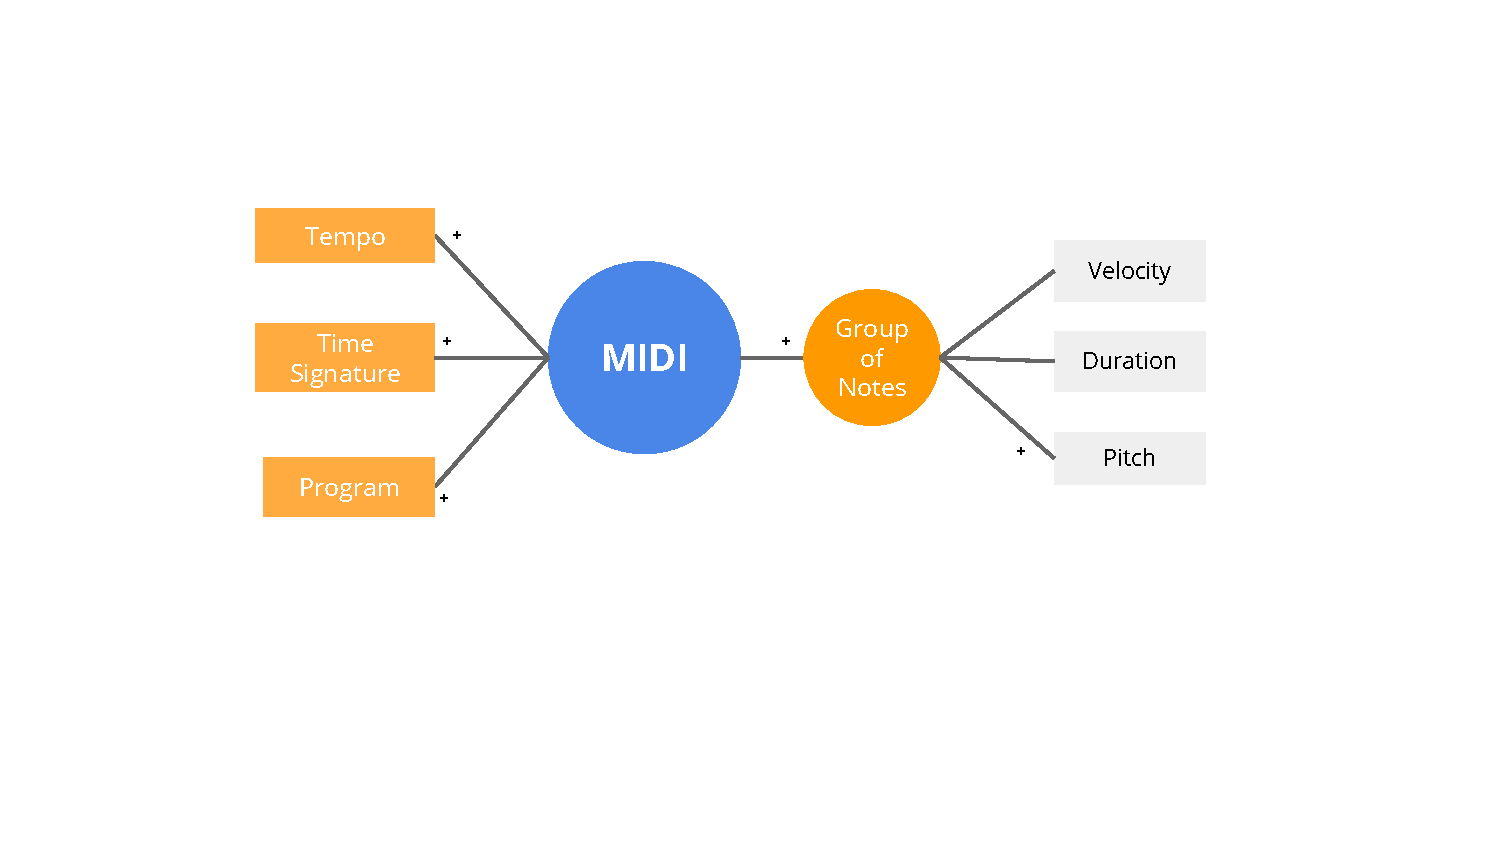
\includegraphics[width=\columnwidth]{figs/schema-midi-graph.pdf}}
 \caption{Schema of the graph generated from MIDI. The \textbf{+} indicates edges representing connections of type many-to-many. The colours represent  different groups of nodes: MIDI $M$ (blue), Content $C$ (orange) among which Notes $N$ have a round shape, and Attributes $A$ (grey). }
 \label{fig:schema-midi-graph}
\end{figure}

\begin{figure*}[ht!]
 \centerline{
 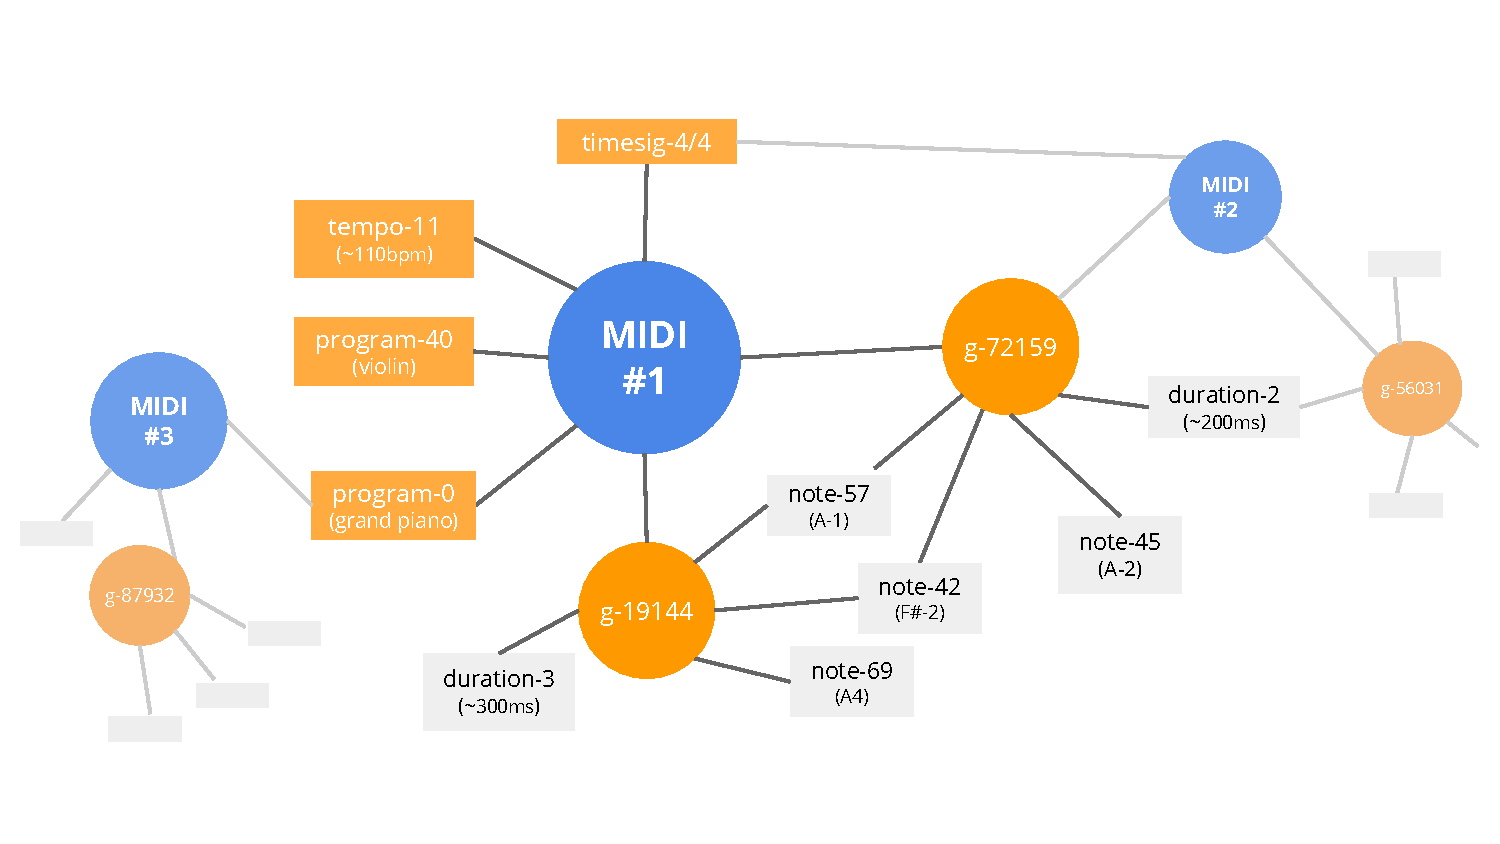
\includegraphics[width=\textwidth]{figs/graph-example.pdf}}
 \caption{MIDI graph example, showing possible connections between MIDI \#1, \#2, and \#3.}
 \label{fig:graph-example}
\end{figure*}

\subsection{Graph to Vectors}
Embeddings are computed on the output graph of the previous process with the \textit{node2vec} algorithm. As more extensively written in \secref{sec:intro-embeddings}, the algorithm simulates random walks on the graph and computes the transition probabilities between nodes, which are mapped into the vector space. In other words, two MIDI files sharing programs, tempos, note groups are more likely to be part of the same random walk and consequently are more likely to be close in the computed embedding space.

In practice, each node in the graph is selected as the starting node for a random walk, occupying its first slot. The second slot will be occupied by one of the nodes directly linked to the first node, according to the probability function. Iteratively, every slot of the random walk will be occupied by one of the neighbours of the previous one. The number of walks to be produced for each node and their length are given parameters. These walks are then processed by \textit{word2vec} as they are sentences.

Following this procedure, a 100-dimensions embedding vector is computed for each node (vertex) of the input graph. Each dimension of the vector cannot be attributed to a specific feature of the described item -- for example, the tempo -- but it rather represents latent features learned by the embedding algorithm. 
We apply a post-processing step in order to keep only the vectors $m \in M$ representing the MIDI files, excluding consequently all the nodes that refer to MIDI messages and attributes.

Such obtained vectors can be then used in input to any algorithm, in tasks such as classification, clustering, and others. In the experiment which will be detailed in the following section, we will use such generated vectors in input to a neural network for classification.
In particular, all vectors used in our experiment have been computed using the following configuration of \textit{node2vec}: walk length = 10, number of walks = 40, window size = 5, number of iterations = 5, p = 0.1, and q=0.1. We also publish as open-source the library for producing MIDI embeddings at [DOUBLE-BLIND CENSURE].
% https://github.com/midi-ld/midi2vec

\section{Evaluation}
\label{sec:evaluation}
We evaluate this strategy in relation to three different goals, involving three different MIDI datasets. These goals are detailed in next sections and consist respectively in predicting the genre, some high-quality metadata, and some user-defined tags.

For each goal, we perform an experiment which rely on a common procedure. 
MIDI embeddings are generated on the dataset using MIDI2vec. A Feed-Forward Neural Network receives the MIDI embeddings as input (100 dimensions) in batches of size 32. The network is detailed in \figref{fig:neural_network}. The set of labels used for training and testing changes according to each experiment. However, it is worth reminding the reader that those labels have not been used in the embedding task, and consequently, they are not directly included in the embedding information. The neural network consists of 3 dense layers. The hidden layers count 100 neurons each and use \textit{ReLU}\endnote{A rectified linear unit (ReLU) is a classic activation function in Deep Learning networks, which return 0 when the input is negative or the input value itself when it is positive. ReLU is widely used because of its simplicity and its empirically demonstrated fast convergence.} as activation function. The output layer uses a sigmoid\endnote{The sigmoid function transforms the input $x$ according to the formula: $$ h_ \theta (x) =  \frac{\mathrm{1} }{\mathrm{1} + e^- \theta^Tx }  $$ It exists between 0 and 1, so it is widely used when probabilities are requested in output. Its step curve shape gives it a behaviour similar to the Heaviside step, but derivable for any input.} as activation function and has a number of neurons equal to the dimension of the vocabulary of labels, which is represented with one-hot encoding. We performed 10-fold cross-validation for training the neural network and we provide as final score the average of the accuracy\endnote{The definition of \textit{accuracy} is ``the closeness of agreement between a test result and the accepted reference value'', i.e. the true value (ISO 5725-1).} computed on every fold.

For the first two goals (\secref{sec:genre-pred} and \ref{sec:metadata-pred}), a further experiment requires a preliminary splitting of the dataset in 10 equal folds, in order to alternatively use 1 of them as test set and the remaining 9 as training set, implementing a complete 10-fold cross-validation (CCV). The embeddings are generated using exclusively the training set, while the vectors representing the MIDI files in the test set are computed \textit{a posteriori} as the mean of the embeddings of their sibling elements in the graph (tempos, programs, note groups, time signatures). Even if this approach is not commonly applied and not equivalent to the result of an embedding learning, we include this simplification with the purpose of demonstrating how graph embedding information is generalisable to unseen data. In the context of this experiment, the reported accuracy refers to the predictions on the test set generated by the neural network trained on the training set.

These experiments are available as notebooks at [DOUBLE-BLIND CENSURE].
% https://github.com/pasqLisena/midi-embs
Furthermore, all models (embeddings) learned for each dataset are also published for supporting research reproducibility [DOUBLE-BLIND CENSURE].
%https://zenodo.org/xxx

\begin{figure}[ht]
\centering
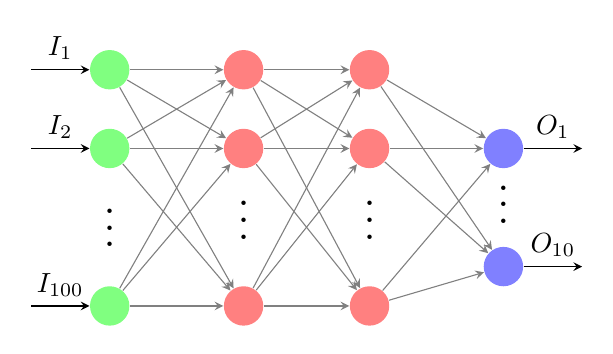
\begin{tikzpicture}[x=1cm, y=1cm, >=stealth]
\foreach \m/\l [count=\y] in {1,2}
{ \node [circle,fill=green!50,minimum size=0.5cm] (input-\m) at (0,2.5-\y) {};}
\foreach \m/\l [count=\y] in {3}
{ \node [circle,fill=green!50,minimum size=0.5cm ] (input-\m) at (0,-1.5) {};}
 \node [neuron missing]  at (0,-0.5) {};
 
\foreach \m [count=\y] in {1,2}
  \node [circle,fill=red!50,minimum size=0.5cm ] (hidden-\m) at (1.7,2.5-\y) {};
\foreach \m [count=\y] in {3}
  \node [circle,fill=red!50,minimum size=0.5cm ] (hidden-\m) at (1.7,-1.5) {};
 \node [neuron missing]  at (1.7,-0.4) {};

\foreach \m [count=\y] in {1,2}
  \node [circle,fill=red!50,minimum size=0.5cm ] (hidden2-\m) at (3.3,2.5-\y) {};
\foreach \m [count=\y] in {3}
  \node [circle,fill=red!50,minimum size=0.5cm ] (hidden2-\m) at (3.3,-1.5) {};
 \node [neuron missing]  at (3.3,-0.4) {};

\foreach \m [count=\y] in {1}
  \node [circle,fill=blue!50,minimum size=0.5cm ] (output-\m) at (5,1.5-\y) {};
  
\foreach \m [count=\y] in {2}
  \node [circle,fill=blue!50,minimum size=0.5cm ] (output-\m) at (5,-\y) {};

 \node [neuron missing]  at (5,-0.2) {};

\foreach \l [count=\i] in {1,2,100}
  \draw [<-] (input-\i) -- ++(-1,0)
    node [above, midway] {$I_{\l}$};

\foreach \l [count=\i] in {1,10}
  \draw [->] (output-\i) -- ++(1,0)
    node [above, midway] {$O_{ \l}$};

\foreach \i in {1,...,3}
  \foreach \j in {1,...,3}
    \draw [->,gray] (input-\i) -- (hidden-\j);

\foreach \i in {1,...,3}
  \foreach \j in {1,...,3}
    \draw [->,gray] (hidden-\i) -- (hidden2-\j);
    
\foreach \i in {1,...,3}
  \foreach \j in {1,...,2}
    \draw [->,gray] (hidden2-\i) -- (output-\j);

%\foreach \l [count=\x from 0] in {Input, Hidden, Ouput}
 % \node [align=center, above] at (\x*2,2) {\l \\ layer};
 
\end{tikzpicture}
    \caption{Scheme of the neural network.}
    \label{fig:neural_network}
\end{figure}

\subsection{Genre Prediction}
\label{sec:genre-pred}
\cite{mckay2010datasetslac} perform a genre classification task on a contextually published SLAC Dataset\endnote{SLAC dataset: \url{http://jmir.sourceforge.net/Codaich.html}}, which contains 250 MIDI files classified according to a two levels taxonomy. The first level includes 5 genre labels (Blues, Classical, Jazz, Rap, Rock), while the second one further specialises each genre by 2 sub-genres, for a total of 10 sub-genre labels. The dataset is perfectly balanced among the classes. Figure \ref{fig:stats-slac} shows a breakdown of the notes, instruments, tempo and time signature found in MIDIs of the SLAC dataset.

\begin{figure}[ht]
    \centering
    \parbox{\linewidth}{
    \subfloat{
        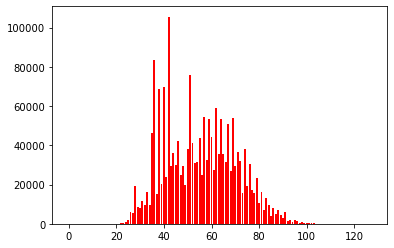
\includegraphics[width=0.45\linewidth]{figs/stat-slac-notes.png}
    }
    ~
    \subfloat{
        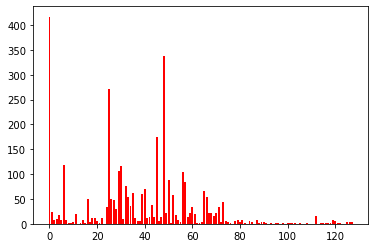
\includegraphics[width=0.45\linewidth]{figs/stat-slac-instruments.png}
   }
   }
    \parbox{\linewidth}{
    \subfloat{
        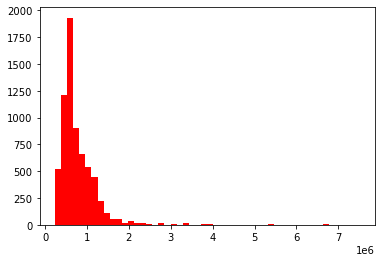
\includegraphics[width=0.45\linewidth]{figs/stat-slac-tempo.png}
    }    ~
    \subfloat{
        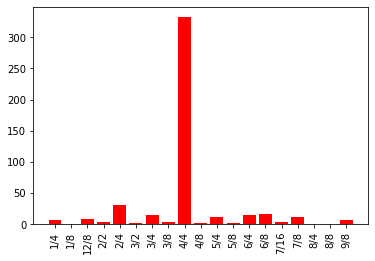
\includegraphics[width=0.45\linewidth]{figs/stat-slac-timesignature.png}
    }
    }
\caption{From left to right and top to bottom, notes, instruments, tempo and time signature of the MIDIs in the SLAC dataset (245 files). The average note is G3; the most frequent instruments (peaks) are acoustic grand piano, acoustic guitar (steel), and string ensemble 1. The average tempo is 771K microseconds per beat (77.8 bpm). The most common time signature is 4/4.}
    \label{fig:stats-slac}
\end{figure}

% A majority of MIDI files contains 10k notes and less than 10 instruments, with just 2 files over 100 and 400 instrument changes (program change event)

We perform a 5-class genre classification experiment as well as a 10-class experiment on the same dataset. In \citep{mckay2010datasetslac}, the authors use different inputs for predicting the genre: symbolic music (S) --which is the MIDI content--, lyrics (L), audio (A), cultural features (C) (tags extracted from the Web) and the multi-modal combination of all of these features (SLAC). In particular, the symbolic information is organised around 111 features (1021 dimensions). Their work has been extended and improved in a more recent paper \citep{mckay2018} including, among others, features about chords and simultaneous notes, for a total of 172 features (1497 dimensions). We will compare our approach with these works, taking into account these 5 variants of features being used.
 The results are reported in \tabref{tab:accuracy-genre}. 

\begin{table}[ht]
    \centering
    \resizebox{\linewidth}{!}{
    \begin{tabular}{|c|c|c|c|}
        \hline
        \multicolumn{2}{|l|}{\textbf{Approach}} &  \textbf{5 classes} &  \textbf{10 classes} \\
        \hline
        \multicolumn{1}{|c|}{\multirow{5}{2cm}{
        \citeauthor{mckay2010datasetslac} \\
        (\citeyear{mckay2010datasetslac})
        }} & S & 85\% & 66\% \\
        \cline{2-4}
        \multicolumn{1}{|c|}{} & L & 69\% & 43\% \\
        \cline{2-4}
        \multicolumn{1}{|c|}{} & A & 84\% & 68\% \\
        \cline{2-4}
        \multicolumn{1}{|c|}{} & C & 100\% & 86\% \\
        \cline{2-4}
        \multicolumn{1}{|c|}{} & SLAC & 99\% & 85\% \\
        \hline
        \multicolumn{2}{|l|}{\cite{mckay2018}} &  93.2\%  &   77.6\% \\
        \hline
        \multicolumn{1}{|c|}{\multirow{6}{*}{MIDI2vec + NN}} & ALL & \textbf{86.4\%} (5.4\%) & \textbf{67.2\%} (7.8\%) \\ 
        \cline{2-4}
        \multicolumn{1}{|c|}{} & *N &      81.6\% (7.6\%) & 62.4\% (9.9\%) \\ 
        \cline{2-4}
        \multicolumn{1}{|c|}{} & *P &      79.6\% (6.8\%) & 61.6\% (8.6\%)\\ 
        \cline{2-4}
        \multicolumn{1}{|c|}{} & *T &      27.2\% (9.5\%) & 18.8\% (9.2\%)\\ 
        \cline{2-4}
        \multicolumn{1}{|c|}{} & *TS &      25.6\% (9.2\%) & 15.2\% (4.4\%)\\ 
        \cline{2-4}
        \multicolumn{1}{|c|}{} & *300 &     79.2\% (7.0\%)& 57.2\% (12.5\%)\\
        \cline{2-4}
        \multicolumn{1}{|c|}{} & CCV &     76.8\% (9.4\%)& 55.2\% (6.5\%)\\
        \hline
    \end{tabular}}
    \caption{Accuracy of the genre classification. The reported values are the average (and standard deviation) of the cross-fold validation. In *N, *P, *T, *TS the embeddings have been computed on the sole notes, programs, tempos and time signature, while ALL includes all of them and *300 uses only the first 300 note-groups. Under CCV, the results of the complete cross-fold validation.}
    \label{tab:accuracy-genre}
\end{table}

Our approach slightly outperforms \citep{mckay2010datasetslac} when only symbolic data are used in input (S), with an accuracy of 86\% for 5-classes and 67\% for 10-classes prediction. In addition, our method outperforms also other variants, namely lyrics (in both classes) and audio (in the 5-classes). The improvements made in \citep{mckay2018} increase these scores of a few percentage points. We believe that the combination of melodic and chords features was crucial in this case and worth to investigate in future work.

The same \tabref{tab:accuracy-genre} shows also the accuracy scores obtained with different variations of the complete model (ALL); these variations compute the embeddings on the sole notes nodes (*N), program nodes (*P), tempo nodes (*T), and time signature nodes (*TS). None of these single features reach the accuracy score of their combination. It is not surprising that *N reaches the higher accuracy among those models, having been computed on a more populated graph -- the number of  \textit{NoteOn}/\textit{NoteOff} events is higher than any other kind of event. Moreover, this study proves the absence of correlation between mono-dimensional features (e.g. tempo) and the classes.
Finally, we trained the embeddings on all features, but taking into account only the first 300 note groups (*300). The experiment shows that reducing the number of vertex in the graph causes lower accuracy scores.

Given the close results between the two best variations (ALL and *N), we studied their statistical significance, in order to understand if these two variations are likely to have the same accuracy mean. In order to do so, we extracted a t statistic computed on a 10x10-fold cross-fold validation, according to \cite{bouckaert2004significance}. Applying this statistic to a Student's t-test, we obtain their p-values, comparing them with the common significance level $\alpha = 0.05$. For the 5 classes classification, the p-value of 0.048 suggests its statistical significance, while this is not confirmed with $p = 0.079$ for the 10 classes case. However, the repeated experiments show always better results for ALL when looking at the average of each 10-fold shuffle, while may happen that *N has punctual higher scores on single folds.

In the complete cross-fold validation (CCV) experiment, the accuracy scores are around 10\% lower. This decrease is mostly due to the difference in computing the vectors of the nodes in the train set (embedding algorithm) and the test set (average of other nodes). However, the results are consistent respect to \textsc{ALL}, suggesting that the system is learning relevant features rather than coincidentally building a smart hashing on the content.

\figref{fig:cm-slac} shows the confusion matrix between the real and the predicted values (configuration ALL). Even if there are no strong patterns, we can state that \textit{Blues} is the genre that attract more negative predictions. This is confirmed by what we see in \figref{fig:tsne-slac}, which contains a 2D visualisation of the vector space realised using the \textit{t-Distributed Stochastic Neighbor Embedding} (t-SNE) algorithm\endnote{Similarly to Principal Components Analysis (PCA), t-SNE maps a high-dimensional space into a low-dimensional one. The algorithm computes the probability that a point A would choose point B as its neighbour, according to a Gaussian probability distribution centred at A.}~\citep{maaten2008visualizing}. The final result is obtained by minimising the differences in this probability when computed on the low-dimensional space with respect to the high-dimensional one. In this figure, items of the same genre look closer in the space, with the \textit{Blues} tracks occupying the central part of the graph, partially overlapping with the area of other genres.
\figref{fig:cm-slac-subgenre} confirms that sub-genres belonging to the same parent genre are easier to be confused.

\begin{figure}[ht]
    \centering
    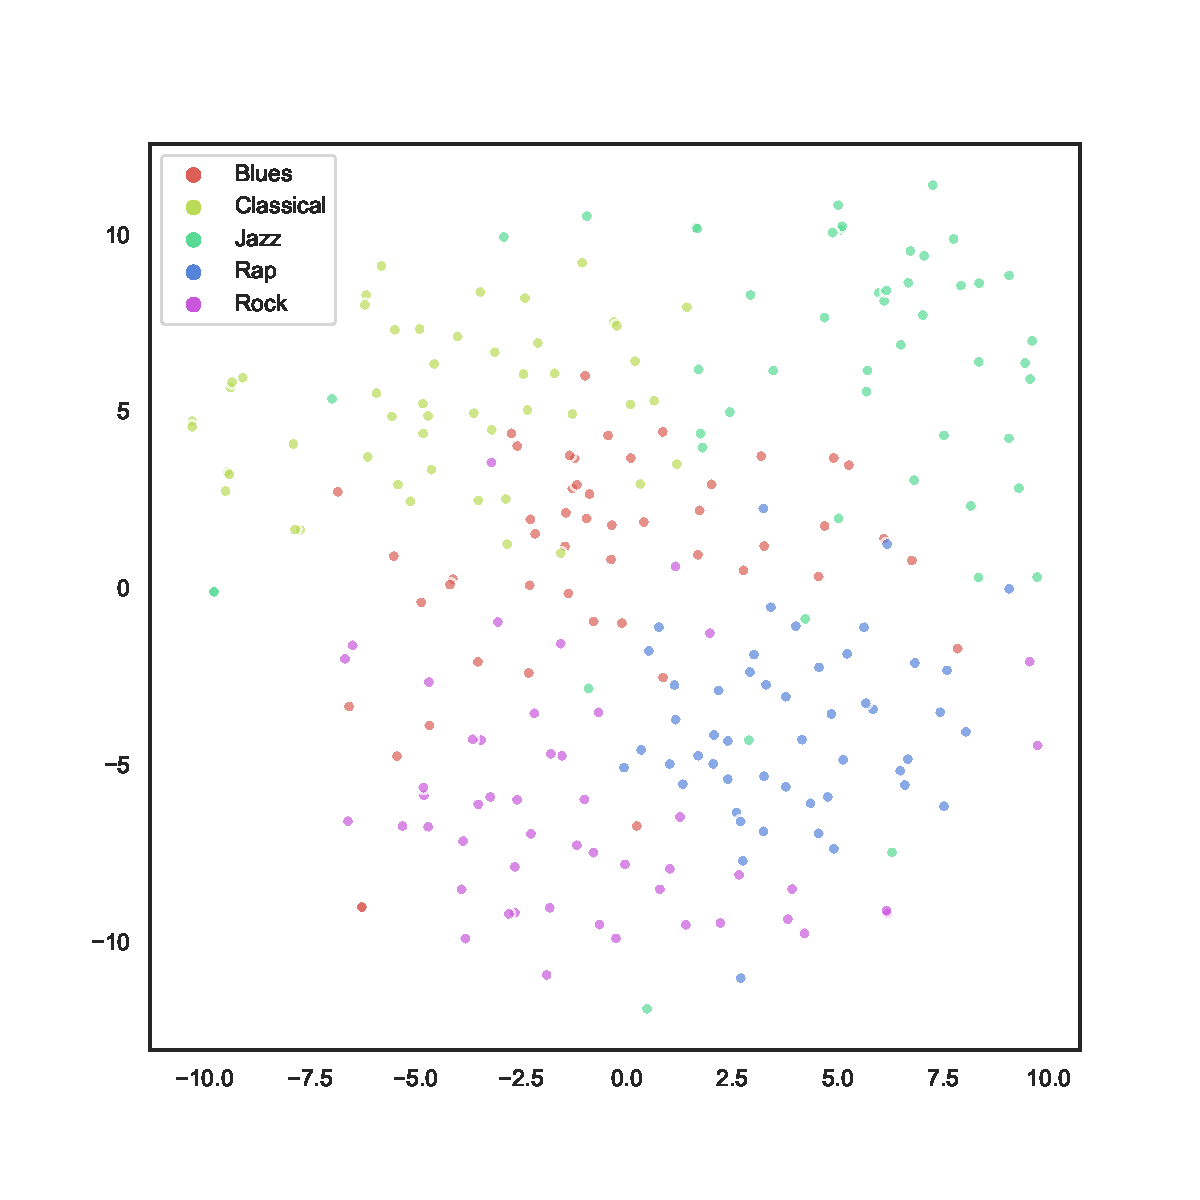
\includegraphics[width=\linewidth]{figs/tsne-slac-genre.pdf}
    \caption{2D representation of the embedding space learned by midi2vec from the SLAC dataset.}
    \label{fig:tsne-slac}
\end{figure}



\begin{figure*}[ht!]
\centering
\subfloat[Genre prediction]{
      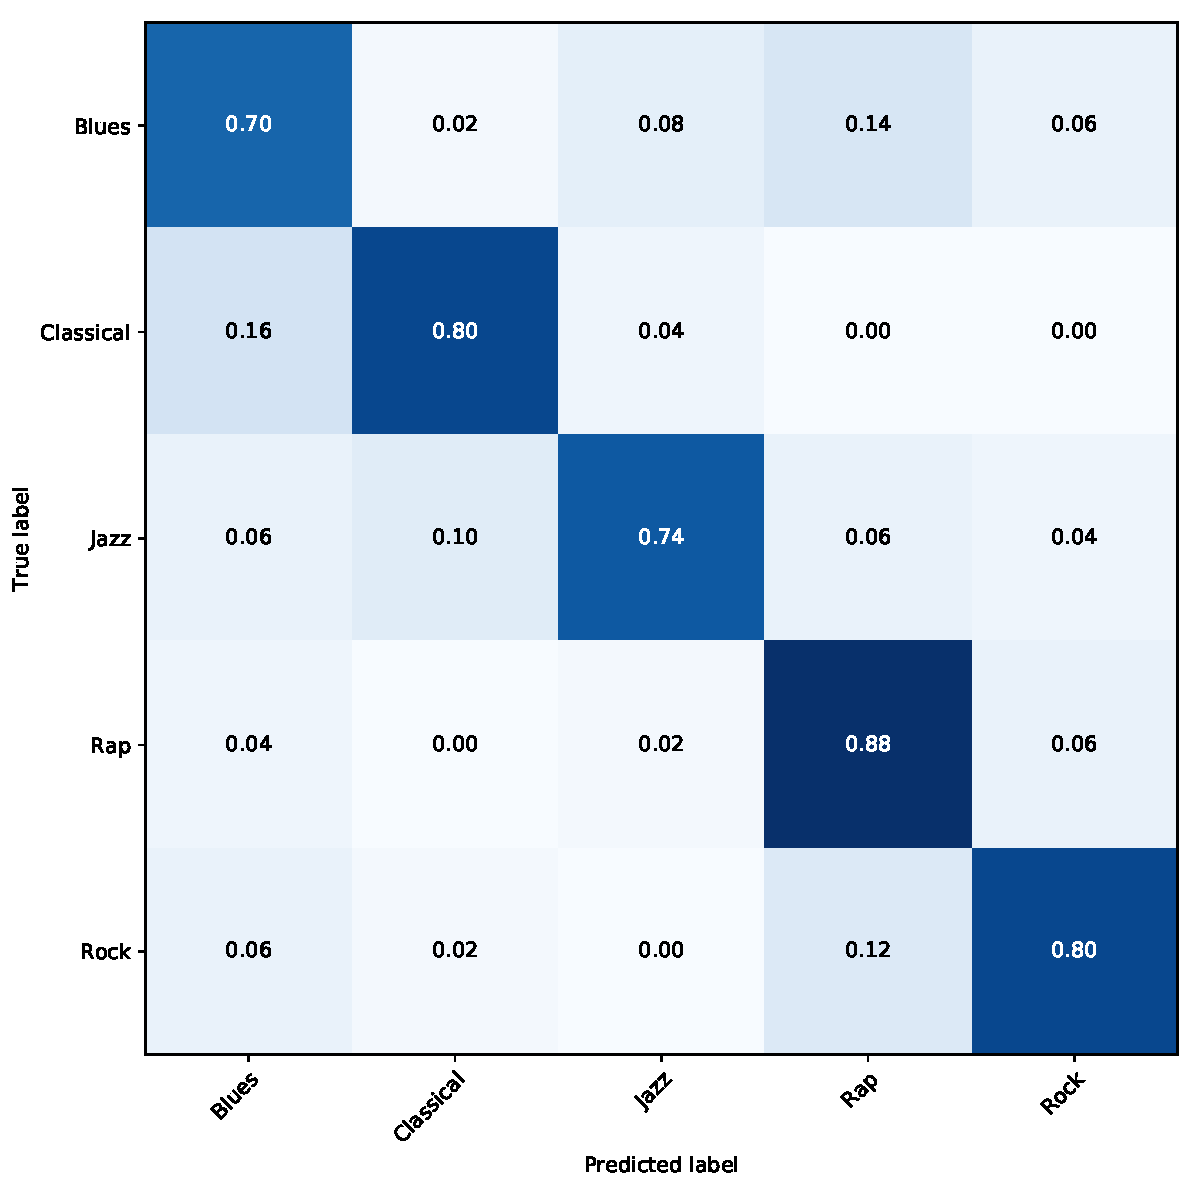
\includegraphics[width=0.47\linewidth]{plot/slac_genre_norm.pdf}
      \label{fig:cm-slac-genre}
}
\hfill
\subfloat[Sub-genre prediction]{
      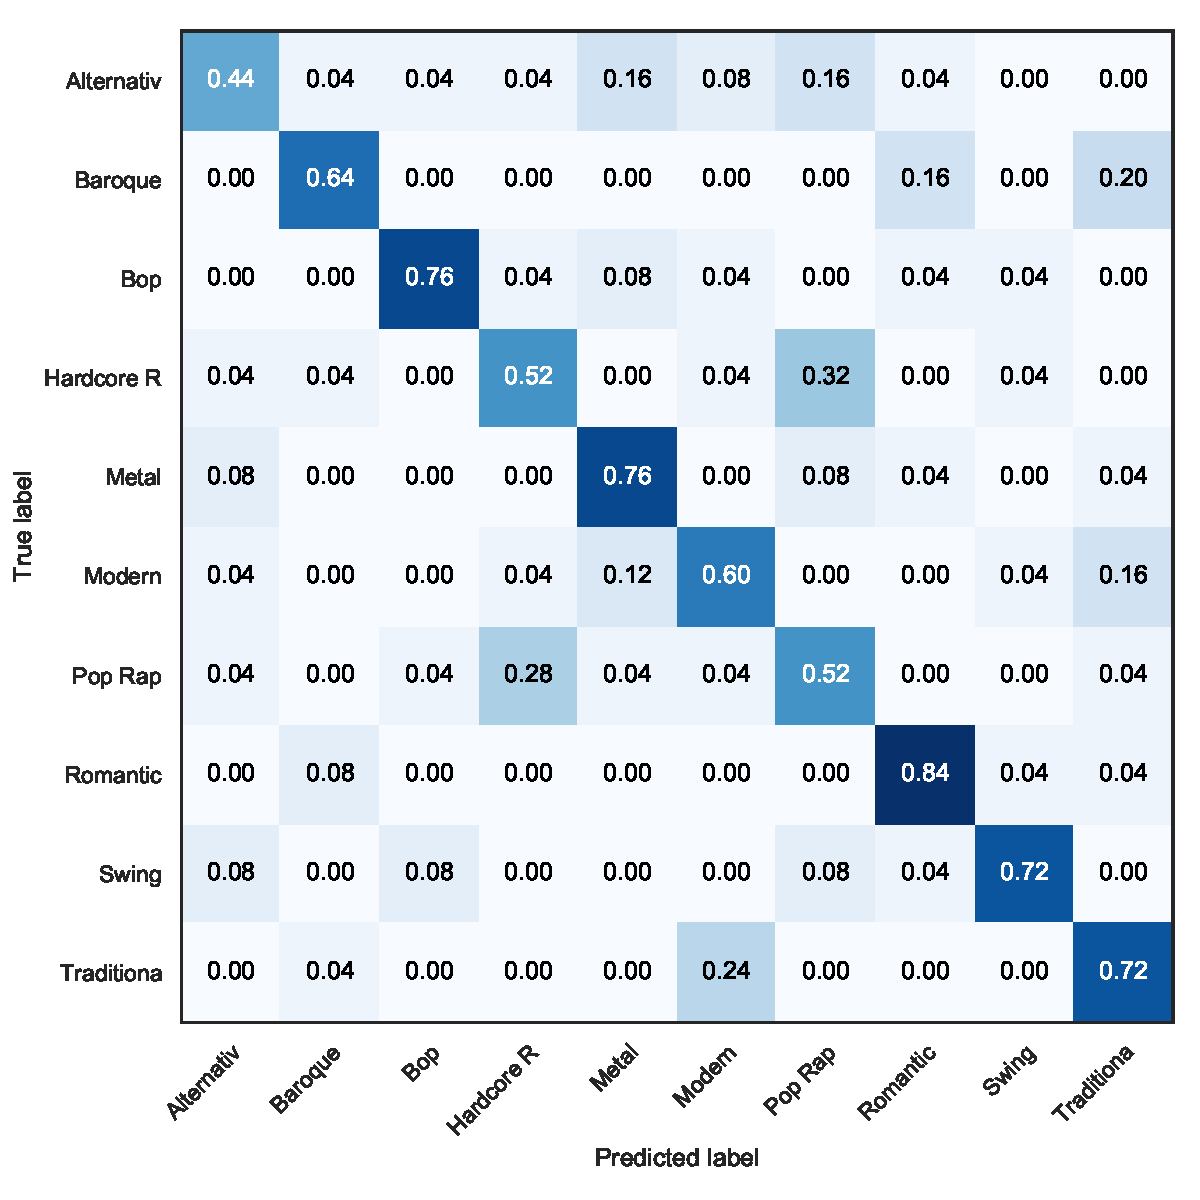
\includegraphics[width=0.47\linewidth]{plot/slac_subgenre_norm.pdf}
      \label{fig:cm-slac-subgenre}
}    
\caption{Confusion matrices of midi2vec predictions for the SLAC dataset.} \label{fig:cm-slac}
\end{figure*}

\begin{figure*}[ht!]
\centering
\subfloat[Composer prediction]{
      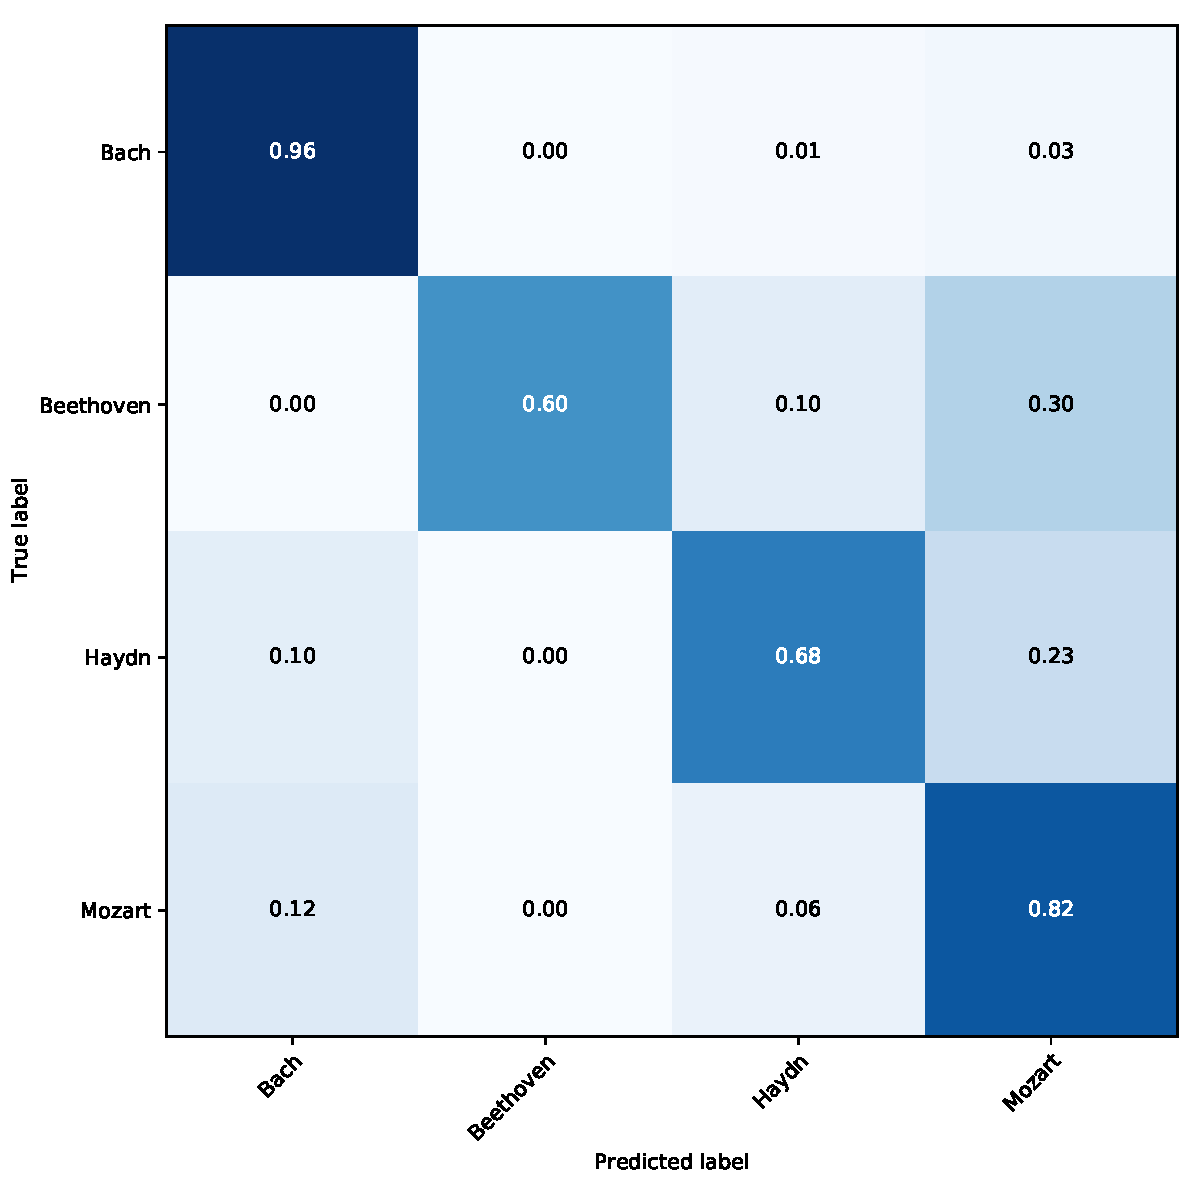
\includegraphics[width=0.47\linewidth]{plot/musedata_composer_norm.pdf}
      \label{fig:cm-doremus-composer}
}
\hfill
\subfloat[Genre prediction]{
      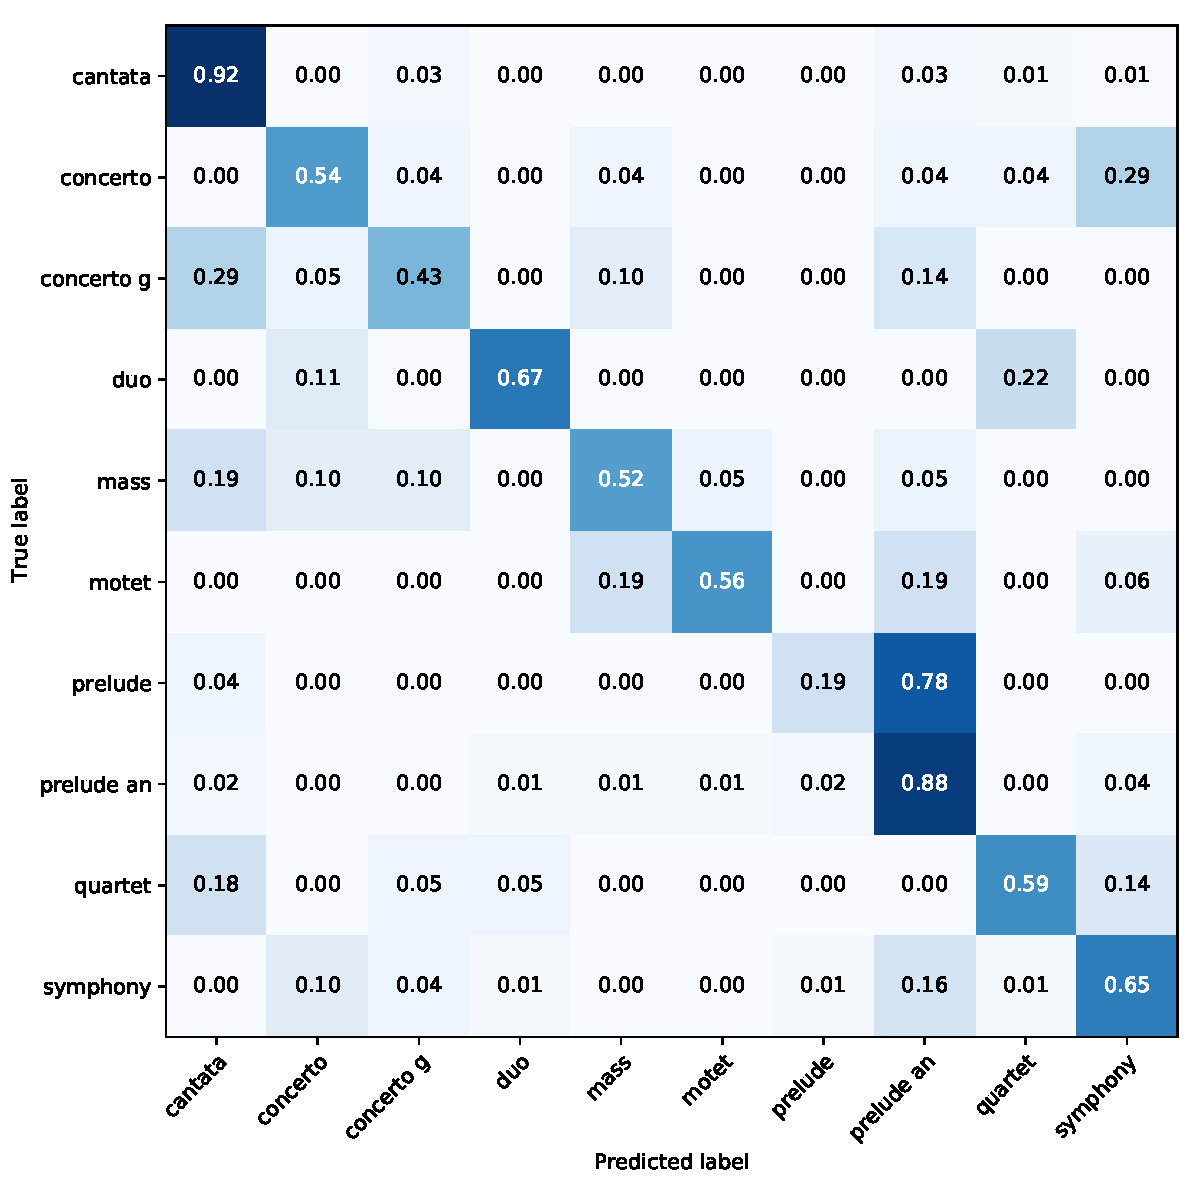
\includegraphics[width=0.47\linewidth]{plot/musedata_genre_norm.pdf}
      \label{fig:cm-doremus-genre}
}    
\\
\subfloat[Instrument prediction]{
      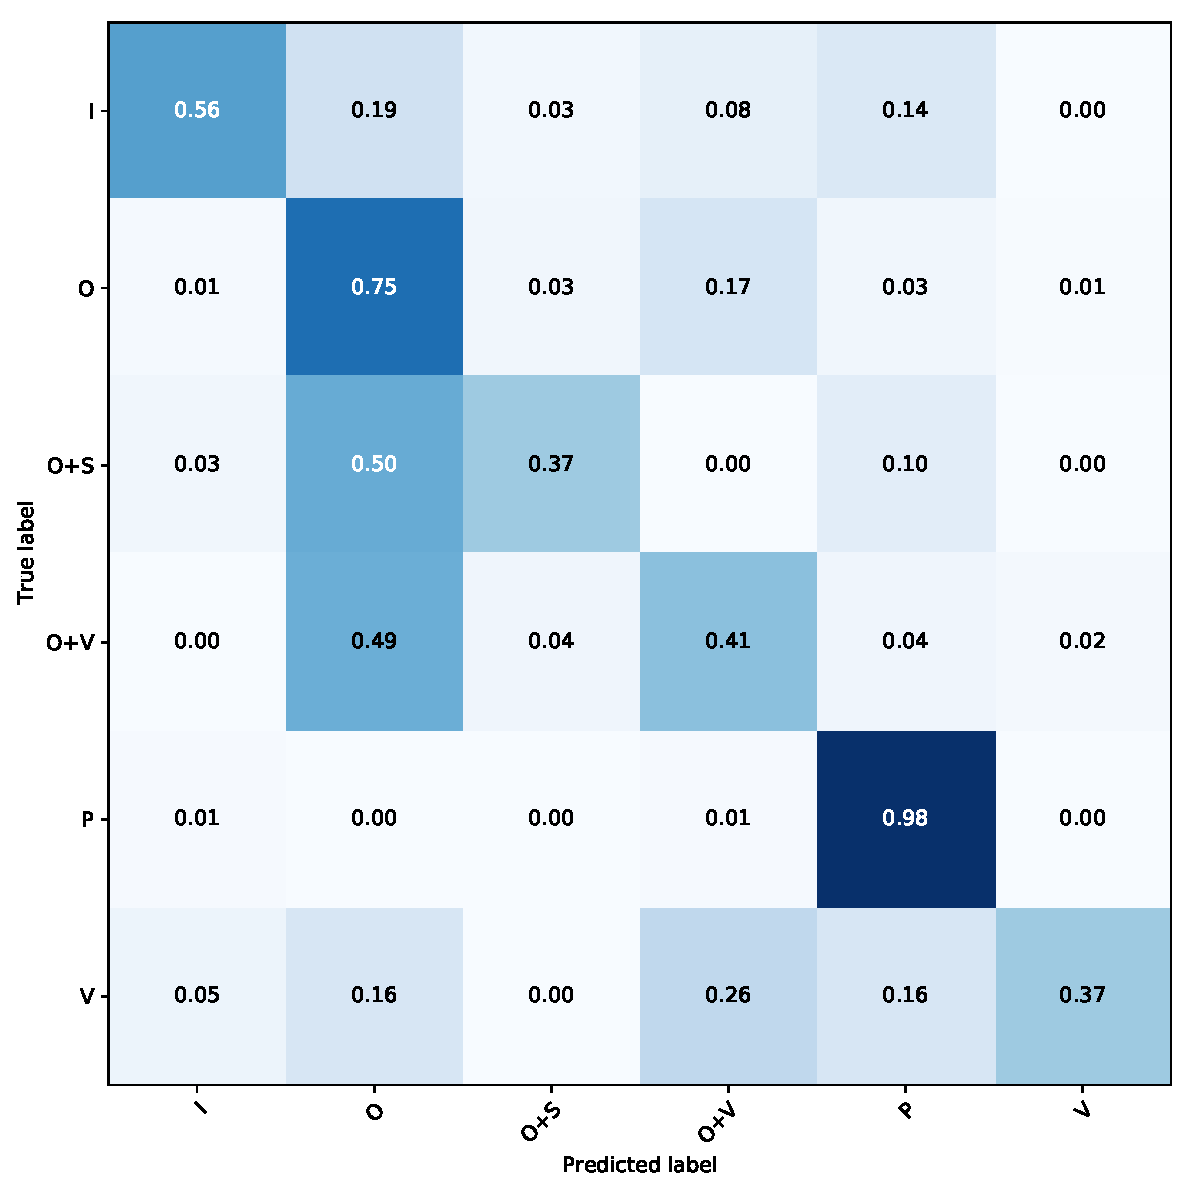
\includegraphics[width=0.47\linewidth]{plot/musedata_instrument_norm.pdf}
      \label{fig:cm-doremus-instr}
}
\hfill
\subfloat[Movement label prediction]{
      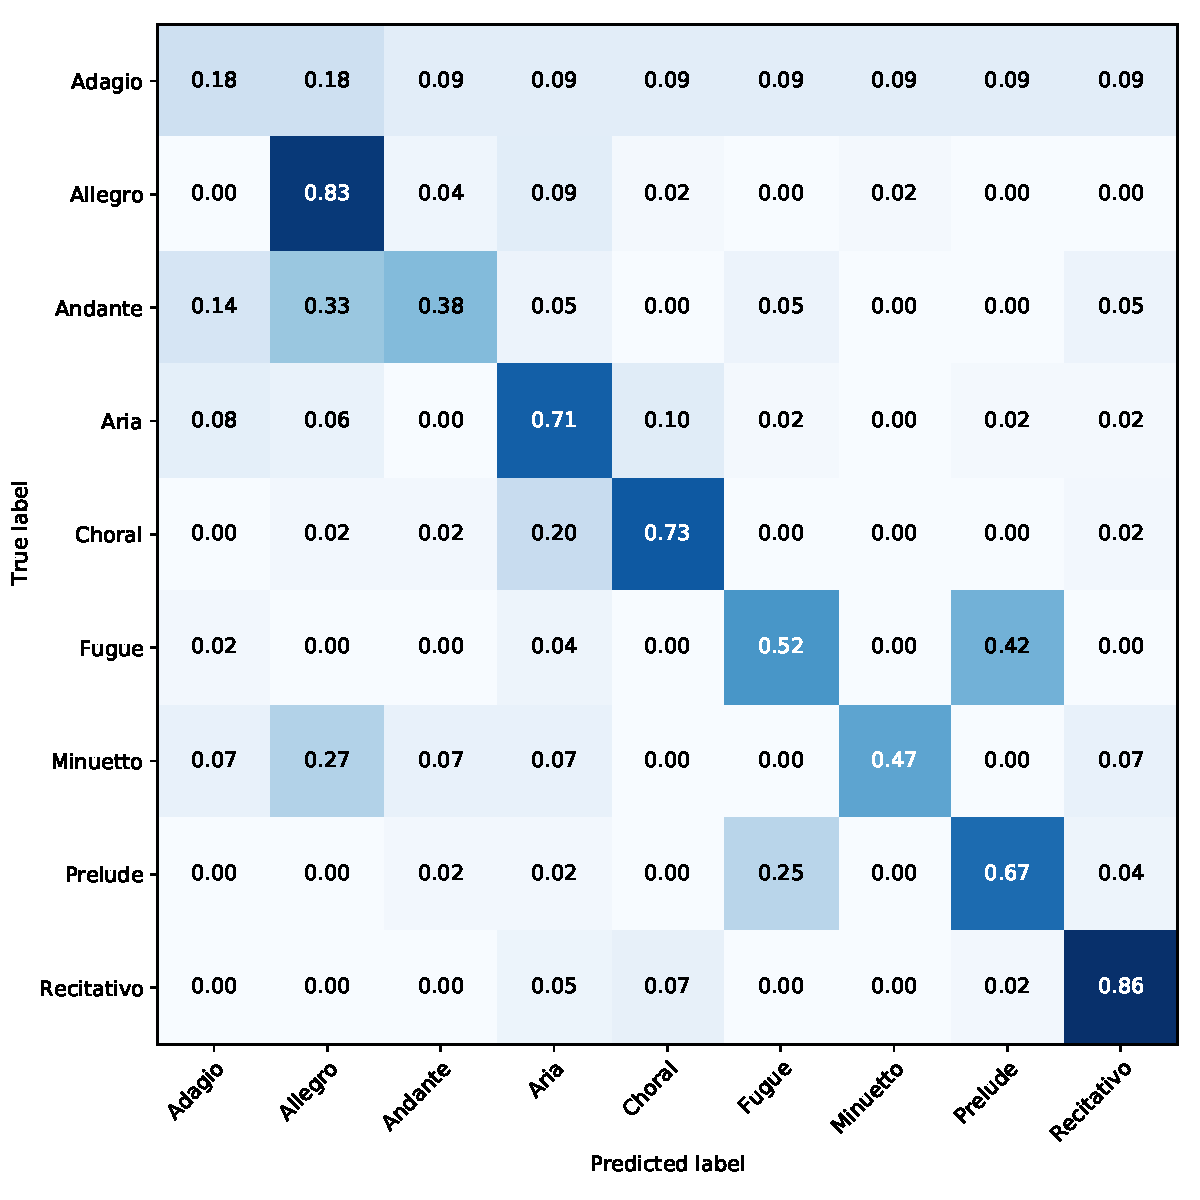
\includegraphics[width=0.47\linewidth]{plot/musedata_mvt_norm.pdf}
      \label{fig:cm-doremus-mvt}
}    

\caption{Confusion matrices of midi2vec predictions for the MuseData dataset. For the instrument predictions (c), the labels are Instrument,  Orchestra, Orchestra + Soloist instrument, Orchestra + Voice, Piano, Voice.} \label{fig:cm-doremus}
\end{figure*}

\subsection{Metadata Prediction}
\label{sec:metadata-pred}
This task consists in predicting a set of metadata from the MIDI, namely the \textit{composer}, the \textit{genre}, the \textit{instrument} and the \textit{movement}.

We started by downloading a corpus of 438 MIDI files from MuseData\endnote{The MuseData dataset is available on the old musedata website: \url{http://old.musedata.org}}. Those files refer to 139 classical music compositions, and each file can represent a specific movement. Figure \ref{fig:stats-musedata} shows a breakdown of the notes, instruments, tempo and time signature found in MIDIs of the MuseData dataset.

\begin{figure}[ht]
    \centering
    \parbox{\linewidth}{
    \subfloat{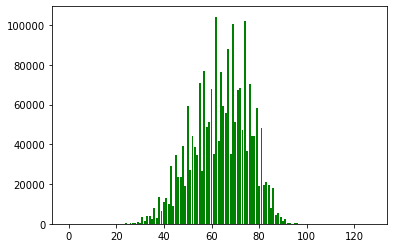
\includegraphics[width=0.45\linewidth]{figs/stat-musedata-notes.png}} 
   \subfloat{        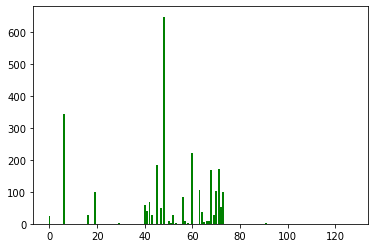
\includegraphics[width=0.45\linewidth]{figs/stat-musedata-instruments.png}} }
    \parbox{\linewidth}{
    \subfloat{
        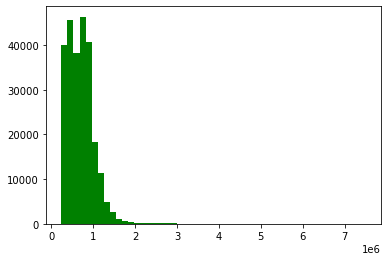
\includegraphics[width=0.45\linewidth]{figs/stat-musedata-tempo.png}
    }
\subfloat{        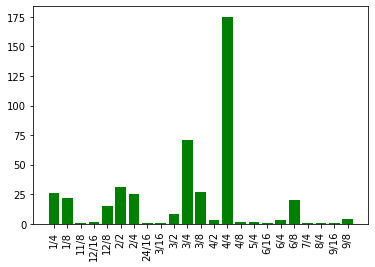
\includegraphics[width=0.45\linewidth]{figs/stat-musedata-timesignature.png}
    }}
    \caption{From left to right and top to bottom, notes, instruments, tempo and time signature of the MIDIs in the MuseData dataset (343 files). The average note is E4; the most frequent instruments (peaks) are the harpsichord and string ensemble 1. The average tempo is 704K microseconds per beat (85.2 bpm). The most common time signature is 4/4, but 3/4 and 2/2 are also frequent.}
    \label{fig:stats-musedata}
\end{figure}

% Frequency of appearance of MIDI events according to their type in the MuseData dataset (343 files). A majority of MIDI files contains less than 500 notes and less than 6 instruments, with just a few files over 35k notes and 30 instruments.}



MuseData provides also some metadata, like the composer name, the scholar catalogue number, a label for the movement. In order to 
obtain further information (i.e. the genre and the played instruments), we have interlinked each composition against the DOREMUS knowledge base~\citep{achichi2018doremus}, a dataset specialised in classical music metadata.

The interlinking process consists of three successive steps:
\begin{itemize}
    \item interlinking of the composer through the exact match on the full name. This limits the candidates for the composition interlinking to the sole compositions of the interlinked composer;
    \item interlinking of the composition through the exact match on the catalogue number;
    \item if no catalogue number match is found, the titles are involved in the process. A title can often contain other kinds of information, such as key, instruments, opus number, etc. For example, the title ``Symphony No. 3 in E-flat Major" contains the order number and the key. For this reason, titles are tokenised through empirical methods based on regular expressions to separate the different parts of the string, used as input of the Extended Jaccard Measure.~\citep{tigrine2015lyam}
\end{itemize}

Every composition can be linked to more than one MIDI file, in the case of works made of multiple movements. The movement labels have been cleaned by removing the order number, the key, the instruments and eventual comments in parentheses. For example, \textit{``1. Allegro in E Major"} becomes simply \textit{``Allegro"}.

The interlinking gives access to precise metadata, mostly coming from controlled vocabularies~\citep{lisena2018vocabularies},
in particular composers (4 classes, i.e. Bach, Beethoven, Haydn, and Mozart), genres (10 classes), and instruments. For this last dimension, given the very large number of possibilities, we decided to reduce the number of classes to 6, including piano \texttt{P}, instrument (other than piano, including also small instrument ensembles) \texttt{I}, voice \texttt{V}, orchestra \texttt{O}, orchestra with voice \texttt{O+V}, and orchestra with instrumental soloist \texttt{O+S}. For instrument prediction, we excluded from the input, 21 MIDI with unknown instrumentation and 3 others which did not fall into any of the previous classes, having a final source dataset of 414 items. 

Furthermore, we consider also the movement label as a feature to predict, considering only those which were occurring more than 10 times. Those labels include tempos (\textit{Allegro}) and musical forms (\textit{Prelude}), for a total of 9 distinct classes on 335 MIDI files. Some of these categories are loosely defined, but we consider them as-is since ambiguity is part of music information and therefore also part of the task. The dataset is not balanced among classes and has a strong presence of Bach works (76\% of the total).

\begin{table*}[]
    \centering
    \begin{tabular}{|c|c|c|c|c|c|}
        \hline
        \textbf{feature} &  \textbf{n. items} &  \textbf{n. classes} &  \textbf{midi2vec}  & \textbf{midi2vec CCV} & \textbf{jSymbolic}\\
        \hline
        composer  &  438 & 4  &   90.4\% (5.8\%) & 88.9\% (15.0\%) &  78.7\% (4.9\%) \\
        \hline 
        genre &      438 & 10  &   71.3\%  (6.4\%) & 58.0\% (16.6\%) & 37.9\% (9.3\%)\\
        \hline
        instrument & 414 & 6  &   65.1\%  (17.5\%) & 48.6 (19.5\%) & 46.1\% (8.6\%) \\
        \hline
        movement &   335 & 9  &   68.3\% (12.7\%) & 54.9 (22.7\%) & 32.4 (6.6\%)\\
        \hline
    \end{tabular}
    
    \caption{For each kind of metadata feature, the table reports the number of items, the number of distinct classes, the average (and standard deviation) accuracy score for midi2vec, midi2vec with complete cross validation, jSymbolic.}
    \label{tab:accuracy-metadata}
\end{table*}

The final accuracy (average of all the fold scores) is reported in \tabref{tab:accuracy-metadata}. The best results are achieved for composer and genre prediction, and good results can be observed for all metadata.
Looking at the confusion matrices:
\begin{itemize}
    \item For the composers, the best results belong to Bach (the most present in the dataset). The two Austrian composers Mozart and Haydn are not surprisingly quite confused with one another, belonging both to the Classicism, differently from Beethoven (Classic-Romantic) and Bach (Baroque)~\citep{rosen1997classical}. The score for Beethoven reflect its under-representation (only 10 tracks) in the dataset (\figref{fig:cm-doremus-composer}); 
    \item The genres are much more specific, with respect to the ones investigated in \secref{sec:genre-pred}. As a consequence, the greatest confusion occurs between couples of very similar genres, such as [\textit{concerto}, \textit{symphony}] and [\textit{prelude}, \textit{prelude and fugue}] (\figref{fig:cm-doremus-genre}). Those genre groups are overlapping also in the t-SNE visualisation in \figref{fig:tsne-musedata};
    \item While the instrument prediction has great results in identifying works for orchestra, piano solo or small ensemble of instruments, it reveals some unreliable classification for voice-only pieces, probably due to the under-representation of the class in the dataset. In the same way, the approach is not able to distinguish compositions for orchestra, orchestra and voice, and orchestra and soloist, all classified under the class \texttt{O} (\figref{fig:cm-doremus-instr});
    \item Even if the movement labels include heterogeneous meaning, the network correctly predicts 7 over 10 items. Some confusion patterns can be spotted. The \textit{Fugue} tag is often predicted as \textit{Prelude}, on the other hand proving a correct genre prediction. The classes representing tempos (e.g. \textit{Adagio} or \textit{Tempo di Minuetto}) are often confused with the most represented class among them (\textit{Allegro}). Some confusion is visible also between the two tags related to singing, \textit{Aria} and \textit{Choral} (\figref{fig:cm-doremus-mvt}).
\end{itemize}

Also in this case, we loose some accuracy (around 12-15\%) when applying the complete cross-validation strategy. In order to have a comparison, we replicated the classification experiment of \cite{mckay2018}, applying to Musedata a SVM classifier trained on the feature vectors computed by jSymbolic\endnote{We also used the jSymbolic vectors in combination with a Neural Network, but obtaining worse performance scores.}. The results show how the features extracted from midi2vec are more capable to discern overlapping classes -- e.g. genres of classical music, movement labels.

All those results should be analysed with a grain of salt, given the absence of balance between classes in the dataset.

\begin{figure}[ht!]
    \centering
    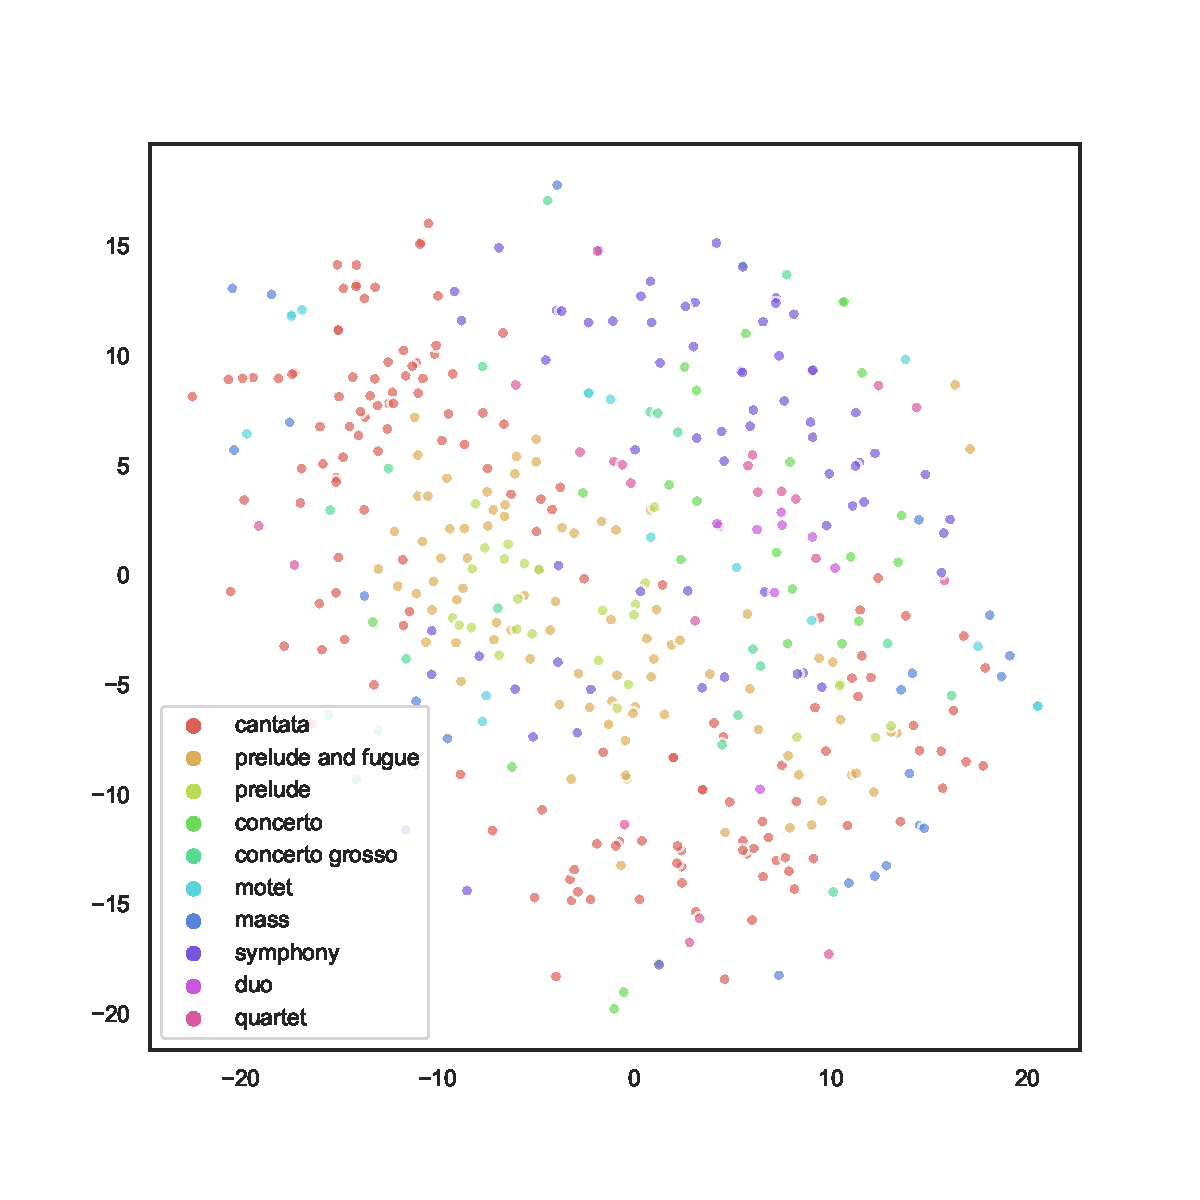
\includegraphics[width=\linewidth]{figs/tsne-musedata-genre.pdf}
    \caption{2D representation of the embedding space learned by midi2vec from the MuseData dataset.}
    \label{fig:tsne-musedata}
\end{figure}

\subsection{Tag Prediction}
The Lakh MIDI Dataset (LMD)\endnote{Lakh MIDI Dataset: \url{https://colinraffel.com/projects/lmd/}} is one of the biggest collections of MIDI which have been realised for research purposes~\citep{raffel2016thesis}. An \texttt{LMD-matched} subset contains 31,034\endnote{The LMD website declares that \texttt{LMD-matched} includes 45,129 MIDIs. However, only 31,034 of them have metadata within a HDF5 file.} MIDI aligned to entries of the Million Song Dataset, providing a set of metadata about the tracks, the albums and the artists. Figure \ref{fig:stats-lakh} shows a breakdown of the notes, instruments, tempo and time signature found in MIDIs of the Lakh dataset.

\begin{figure}[ht]
    \centering
    \parbox{\linewidth}{
    \subfloat{
        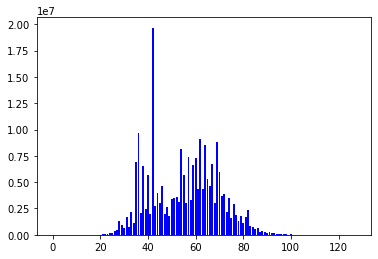
\includegraphics[width=0.45\linewidth]{figs/stat-lakh-notes.png}
    }
    \subfloat{
        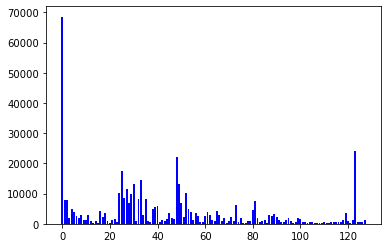
\includegraphics[width=0.45\linewidth]{figs/stat-lakh-instruments.png}
    }}
    \parbox{\linewidth}{
    \subfloat{
        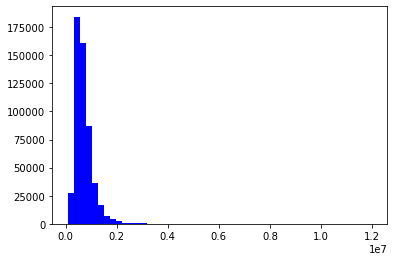
\includegraphics[width=0.45\linewidth]{figs/stat-lakh-tempo.png}
    }     
    \subfloat{
        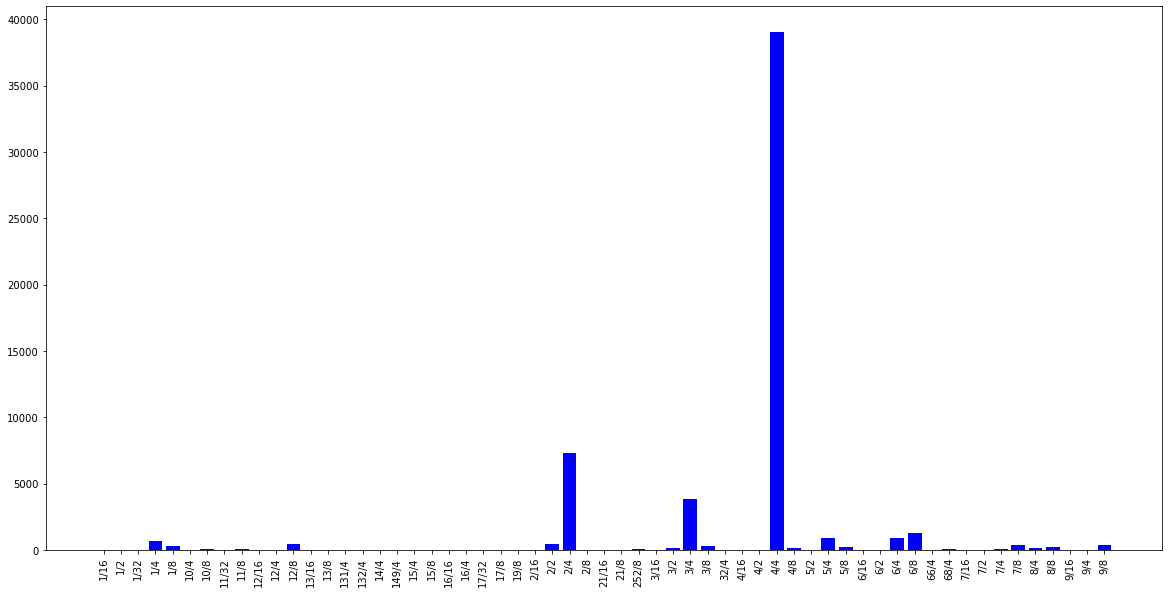
\includegraphics[width=0.45\linewidth]{figs/stat-lakh-timesignature.png}}}m
    \caption{From left to right and top to bottom, notes, instruments, tempo and time signature of the MIDIs in the Lakh dataset (30,732 files). The average note is G3; the most frequent instruments (peaks) are the acoustic grand piano, acoustic guitar (steel), string ensemble 1, and bird tweet. The average tempo is 705K microseconds per beat (85.0 bpm). The most common time signature is 4/4; 2/4 and 3/4 are also frequent.}
    \label{fig:stats-lakh}
\end{figure}

% Frequency of appearance of MIDI events according to their type in the Lakh dataset (30,732). MIDI files of up to 15k notes and less than 10 instruments are very frequent, with just a few files over 55k notes and up to 2610 instrument changes.

We extracted from \texttt{LMD-matched} two kinds of tags, coming respectively from MusicBrainz\endnote{MusicBrainz: \url{https://musicbrainz.org/}} and The Echo Nest\endnote{The Echo Nest: \url{http://the.echonest.com/}}. The former group is a mix of terms which may refer to genres -- i.e. \textit{classic pop} -- or to nationalities -- \textit{British} -- while the latter group is more homogeneous in representing genres. Both kinds of tags refer more to the artist rather than to the exact track.

Differently from the experiment in \secref{sec:metadata-pred}, the size of the dataset allows to further filter the data in order to extract a balanced dataset. In particular, we select all distinct classes which are represented by at least 50 instances. For each of these classes, we randomly select 50 instances. \tabref{tab:accuracy-tag} shows the accuracy for the predictions, measured through 10-fold cross-validation, together with the number of classes (distinct tags) against which we run the classification. In addition, in the table are reported the accuracy scores obtained by an SVM classifier build on top of jSymbolic. The comparison of this results reveals that latent features can largely boost the performance in tag classification, with evident benefit in real world scenarios like automatic tag prediction.

\begin{table*}[]
\centering
\begin{tabular}{|c|c|c|c|c|}
\hline
\textbf{feature} & \textbf{n. items} & \textbf{n. classes} & \textbf{midi2vec} & \textbf{jSymbolic} \\ \hline
MusicBrainz & 2400 & 48 & 39.7\% (2.8\%) & 3.7\% (1.4\%)\\ \hline
EchoNest & 6800 & 136 & 32.5\% (1.9\%) & 1.4\% (0.4\%)\\ \hline

\end{tabular}
\caption{For each kind of tag feature, the table reports the number of items, the number of distinct classes, the average (and standard deviation) accuracy score for midi2vec and jSymbolic.}
\label{tab:accuracy-tag}
\end{table*}

The confusion matrices are shown in \figref{fig:cm-lakh}. Among the most wrongly predicted MusicBrainz classes, we find a strong presence of nationality tags (\textit{British}, \textit{Italian}, \textit{UK}, etc.).
The consistent number of classes do not let us detect patterns in the confusion matrix, in which the best values are however concentrated in the diagonal of corrected predictions.
In order to overcome this issue, we report in \tabref{tab:confused-lakh} the most frequent wrong predictions. For MusicBrainz tags, the list includes loosely defined genres (\textit{easy listening}, \textit{ccm}), one evident error (line 6.), together with couples of tags which can be considered similar or overlapping (1., 3., 7.). Looking at EchoNest tags, all pairings are meaningful, involving similar or related genres. This data gives us more confidence that the neural network is learning music-relevant features, which are well represented through graph embeddings.

\begin{table}[ht]
\resizebox{\linewidth}{!}{
\begin{tabular}{rlll}
\textbf{tag} & \textbf{ground truth} & \textbf{predicted} & \textbf{\%} \\ \hline
MusicBrainz 1. & ballad & folk rock & 12 \\
 2. & blues-rock & ccm & 12 \\
 3. & classic rock & british invasion & 12 \\
 4. & cool jazz & ccm & 10 \\
 5. & easy listening & classic rock & 12 \\
 6. & flamenco & british invasion & 12 \\
 7. & folk rock & ballad & 10 \\ \hline
EchoNest 8. & orchestra & requiem & 10 \\
 9. & progressive trance & hard trance & 10 \\
 10. & ragtime & jazz & 10 \\
 11.& requiem & orchestra & 10 \\
 12. & techno & tech house & 10
\end{tabular}
}
\caption{Most frequent prediction errors for tag classification, with the percentage of cases over the total of the class}
\label{tab:confused-lakh}
\end{table}


\begin{figure*}[ht!]
\centering
\subfloat[MusicBrainz Tag prediction]{
      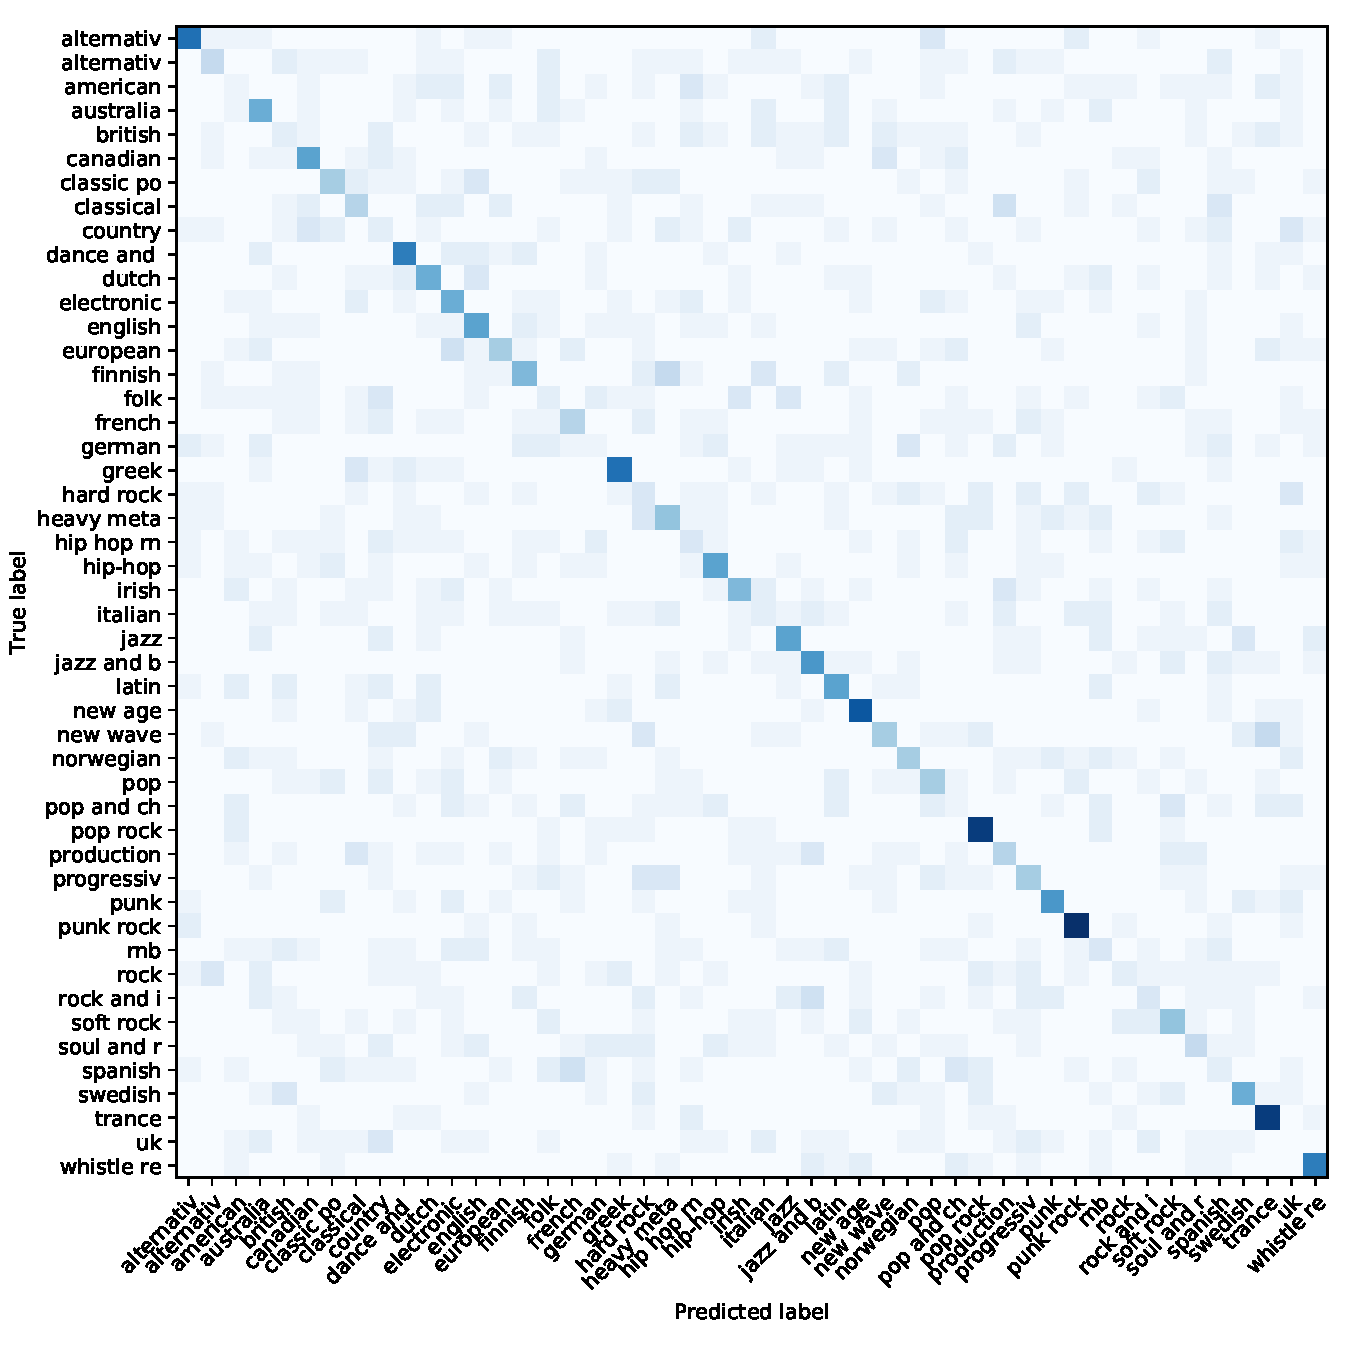
\includegraphics[width=0.47\linewidth]{plot/lakh_mbz_norm.pdf}
      \label{fig:cm-lakh_mbz}
}
\hfill
\subfloat[The Echo Nest Tag prediction]{
      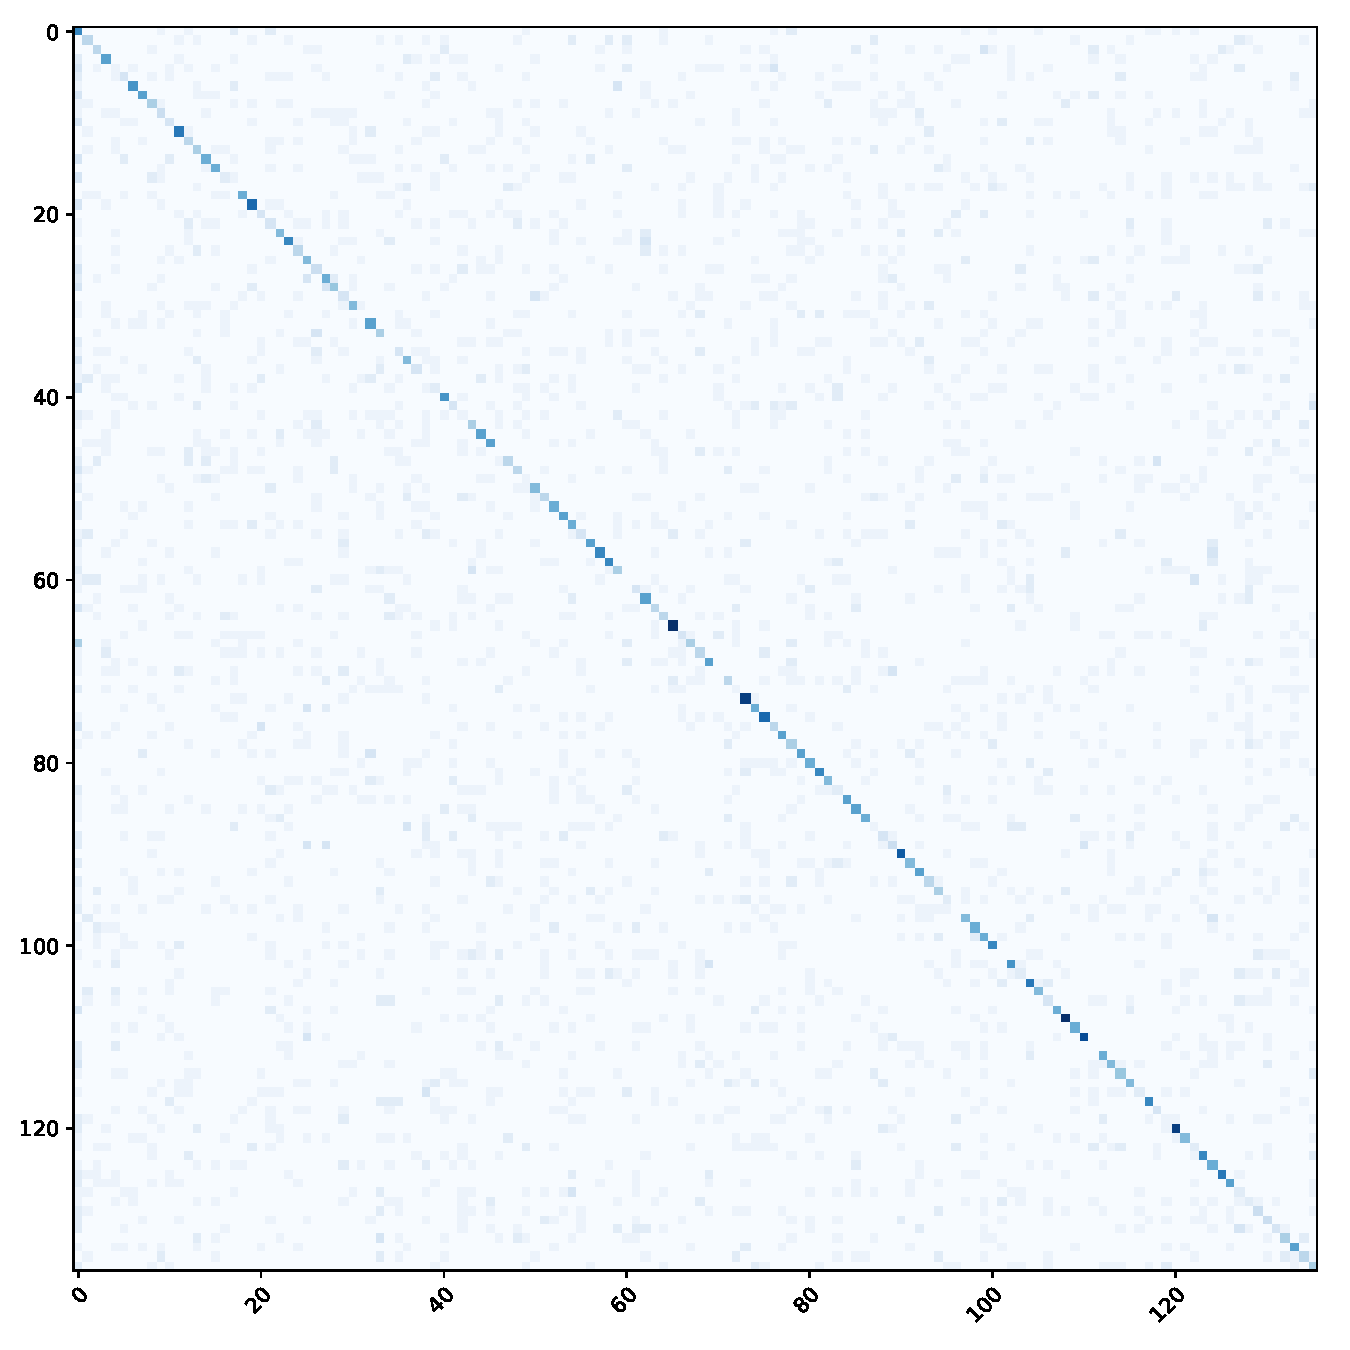
\includegraphics[width=0.47\linewidth]{plot/lakh_echo_norm.pdf}
      \label{fig:cm-lakh_echo}
}    
\caption{Confusion matrices of midi2vec predictions for the Lakh dataset.} \label{fig:cm-lakh}
\end{figure*}

\section{Conclusion and Future Work}
\label{sec:conclusion}
% \todo[inline]{Extend to make a skeptical point about using embeddings for everything--in particular this task}
In this paper, we hypothesise that symbolic music content in MIDI files, and its embedding representation in vector space, are a powerful tool for automated metadata classification tasks. Traditionally, applications of machine learning to this problem have encountered limitations in feature selection, and more recent embedding-based techniques have been only used for other tasks (e.g. music generation) or on different data (e.g. music metadata). In this paper, we propose MIDI2vec, a method to represent MIDI content as a graph and, subsequently, in a vector space through learning graph embeddings. We gather evidence that our hypothesis holds: MIDI2vec embeddings were successful in metadata classification, obtaining comparable performances to state-of-art methods based on feature extraction from symbolic music, with the added advantages of scalability, automating feature engineering, and reducing the required dimensions by one order of magnitude.

We plan on improving this work in various ways. Currently, the library deals with the unpitched notes in MIDI Channel 10 (reserved to percussion) as they have a pitch; a separated branch of the graph will be reserved to percussion notes in the future, on order to distinguish them from the other ones while still taking them into account.

Being transformed into a flat graph, the MIDI content loses in MIDI2vec all time-based information, with the only exception of simultaneity. Given the importance of melodic patterns in a music piece, future work would investigate how this work can deal with note sequences. We plan to investigate a few different strategies.
First, sequences of notes may be encoded similarly to the simultaneous notes groups and included in MIDI2vec as a fifth node type.
A second strategy may rely upon the inclusion in the graph embedding process of sequence embeddings like Sequence Graph Transform (SGT), which is capable to short- and long- term sequence features~\citep{ranjan2016sequence}.
It is possible to think of MIDI file as a \textit{temporal graph}, in which the information (currently played notes, tempo, playing instruments, etc.) is evolving over time, and apply to such a graph temporal node embeddings strategies~\citep{singer2019temporalgraphs}.
Finally, another study may combine MIDI2vec with other feature extraction techniques -- e.g. the previously cited \cite{mckay2018} -- in an ensemble system, in order to exploit the best of the two methods.

A MIDI ontology and a corpus of over 300 thousand MIDI in RDF format have been presented in~\citep{merono2018semantic_midi}. Despite being an interesting target for MIDI2vec, the extraction of crucial information (like the duration of a note) from the dataset is hard. In the current version, the ontology faithfully reproduces the event structure of the MIDI files, while significant edges -- e.g. among simultaneous notes or consecutive events -- are missing. Still, the MIDI2vec approach does not exploit edges between consecutive groups of notes, while they may potentially impact on the performances. We plan to extend or map the MIDI ontology in order to solve this issue and enable MIDI2vec for working on such corpus, e.g. to perform link discovery and knowledge graph completion. Moreover, it would be interesting to extend this approach to other symbolic music notation formats, namely MusicXML.

According to some intuition from other works in the genre classification field~\citep{Cataltepe2007}, the computation should not necessarily involve the full length of the track. Experiments with different time spans or sample sizes among the graph edges can help in detecting a trade-off between the performances and the embedding computation time. Recent approaches for including literal values in graph embeddings~\citep{cochez2018literals, kristiadi2018literale} could be included in MIDI2vec, in order to avoid any arbitrary choice that value-partitioning implies. Finally, we will use MIDI2vec in more applied contexts, such as the task of knowledge graph completion in knowledge bases with incomplete metadata entries \citep{merono2017midi}.

%%%%%%%%%%%%%%%%%%%%%%%%%%%%%%%%%%%%%%%%%%%%%%%%%%%%%%%%%%%%%%%%%%%%%%%%%%%%%%%%
% Please do not touch.
% Print Endnotes
\IfFileExists{\jobname.ent}{
   \theendnotes
}{
   %no endnotes
}

% \section*{Acknowledgements}

% We want to thank Peter Bloem for his advice on strategies for class sampling.

% Any acknowledgements must be headed and in a separate paragraph,
% placed after the main text but before the reference list.

% \interlinepenalty=1000000
\bibliography{TISMIRtemplate}


\end{document}
